% ------------ begin cheatsheet
\documentclass[a4paper]{article}
\usepackage[a4paper,margin=0.1in,landscape]{geometry}
\usepackage{multicol}

\usepackage{amsmath, amssymb}
\usepackage[inline]{enumitem}
\usepackage{graphicx}

\usepackage{ulem}
\usepackage{makecell}

% horizontal list
\newlist{hlist}{enumerate*}{1}
\setlist[hlist]{label={}, afterlabel={}, itemjoin={{ \textbar{} }}}

% math
\newcommand{\abs}[1]{\left\lvert#1\right\rvert}

% envs
\newcommand{\oli}[1]{\begin{enumerate*}[label=(\arabic*)]#1\end{enumerate*}}

\graphicspath{ {./images/} }
\pagestyle{empty}
\setlength{\columnseprule}{0.3pt}

% reduce spacing before and after headers
\newcommand{\uppercaseandunderline}[1]{\uline{\uppercase{#1}}}

\makeatletter
\renewcommand{\section}{
  \@startsection{section}{1}{0pt}{1ex}{1.2ex} {\raggedleft\normalfont\large\bfseries\uppercaseandunderline}}
\renewcommand{\subsection}{
  \@startsection{subsection}{2}{0pt}{1ex}{1.2ex} {\raggedleft\normalfont\normalsize\bfseries\fbox}}
\renewcommand{\subsubsection}{
  \@startsection{subsubsection}{3}{0pt}{1ex}{0.8ex} {\raggedleft\normalfont\small\bfseries\uline}}
\renewcommand{\paragraph}{
  \@startsection{paragraph}{4}{0pt}{1.5ex}{-0.8em}{\normalfont\bfseries}}
% ------------ end cheatsheet

% ------------ begin code
\usepackage{xcolor}
\definecolor{dkgreen}{rgb}{0,0.6,0}
\definecolor{gray}{rgb}{0.5,0.5,0.5}
\definecolor{mauve}{rgb}{0.58,0,0.82}
\definecolor{lg}{rgb}{0.9,0.9,0.9}

% code environment
\usepackage{listings}
\lstset{
  %frame=tb, % adds top and bottom border
  aboveskip=1mm,
  belowskip=1mm,
  showstringspaces=false,
  columns=flexible,
  basicstyle={\small\ttfamily},
  numberstyle=\color{gray},
  keywordstyle=\color{blue}\textbf,
  commentstyle=\color{dkgreen},
  stringstyle=\color{mauve},
  breaklines=true,
  breakatwhitespace=true,
  backgroundcolor=\color{lg},
  tabsize=4
}
\newcommand{\ic}[1]{\lstinline{#1}}

% ------------ end code

% CS2102 symbols
\usepackage{ifsym}
\DeclareMathOperator{\leftjoin}{\scriptscriptstyle \textifsym{d|><|} \displaystyle}
\DeclareMathOperator{\rightjoin}{\scriptscriptstyle \textifsym{|><|d} \displaystyle}
\DeclareMathOperator{\fulljoin}{\scriptscriptstyle \textifsym{d|><|d} \displaystyle}
\newcommand{\dangle}[1]{\mathrm{dangle}(#1)}
\newcommand{\nullrel}[1]{\mathrm{null}(#1)}

\begin{document}
\small
\setlength{\abovedisplayskip}{0pt}
\setlength{\belowdisplayskip}{0pt}
\setlength{\abovedisplayshortskip}{0pt}
\setlength{\belowdisplayshortskip}{0pt}
\lstset{language=SQL}
\begin{multicols*}{3}
  \part*{\centering \underline{CS2102}}
\section*{DBMS}
  \subsection*{Challenges} \noindent
    Want
    \begin{itemize}[leftmargin=*]
      \item (Efficiency) Fast access to information in huge volumes of data
      \item (Transactions) ``All-or-nothing'' changes to data
      \item (Data integrity) Parallel access and changes to data
      \item (Recovery) Fast and reliable handling of failures
        \begin{itemize}[leftmargin=*]
          \item 
            \begin{hlist}
              \item HDD/SSD/system crash
              \item Power outage
              \item Network disruption
            \end{hlist}
        \end{itemize}
      \item (Security) Fine-grained data access rights
    \end{itemize}
  \subsection*{File-based data management}
    \begin{itemize}[leftmargin=*]
      \item Complex, low-level code
      \item Often similar requirements across different programs
    \end{itemize}
    \paragraph{Problems}
      \begin{hlist}
        \item High development effort
        \item Long development times
        \item Higher risk of (critical) errors
      \end{hlist}
  \subsection*{Transaction}
    \begin{itemize}[leftmargin=*]
      \item Finite sequence of database operations (reads and/or writes)
      \item Smallest logical unit of work from an application perspective
    \end{itemize}
    Each transaction T satisfies the following ACID properties:
    \begin{itemize}[leftmargin=*]
      \item Atomicity: either all effects of T are reflected in the database or none
      \item Consistency: Execution of T guarantees to yield a correct state of the database
      \item Isolation: Execution of T is isolated from the effects of concurrent transactions
      \item Durability: After the commit of T, its effects are permanent even in case of failures
    \end{itemize}
  \subsection*{Concurrent Execution}
    \subsubsection*{Common problems} \noindent
      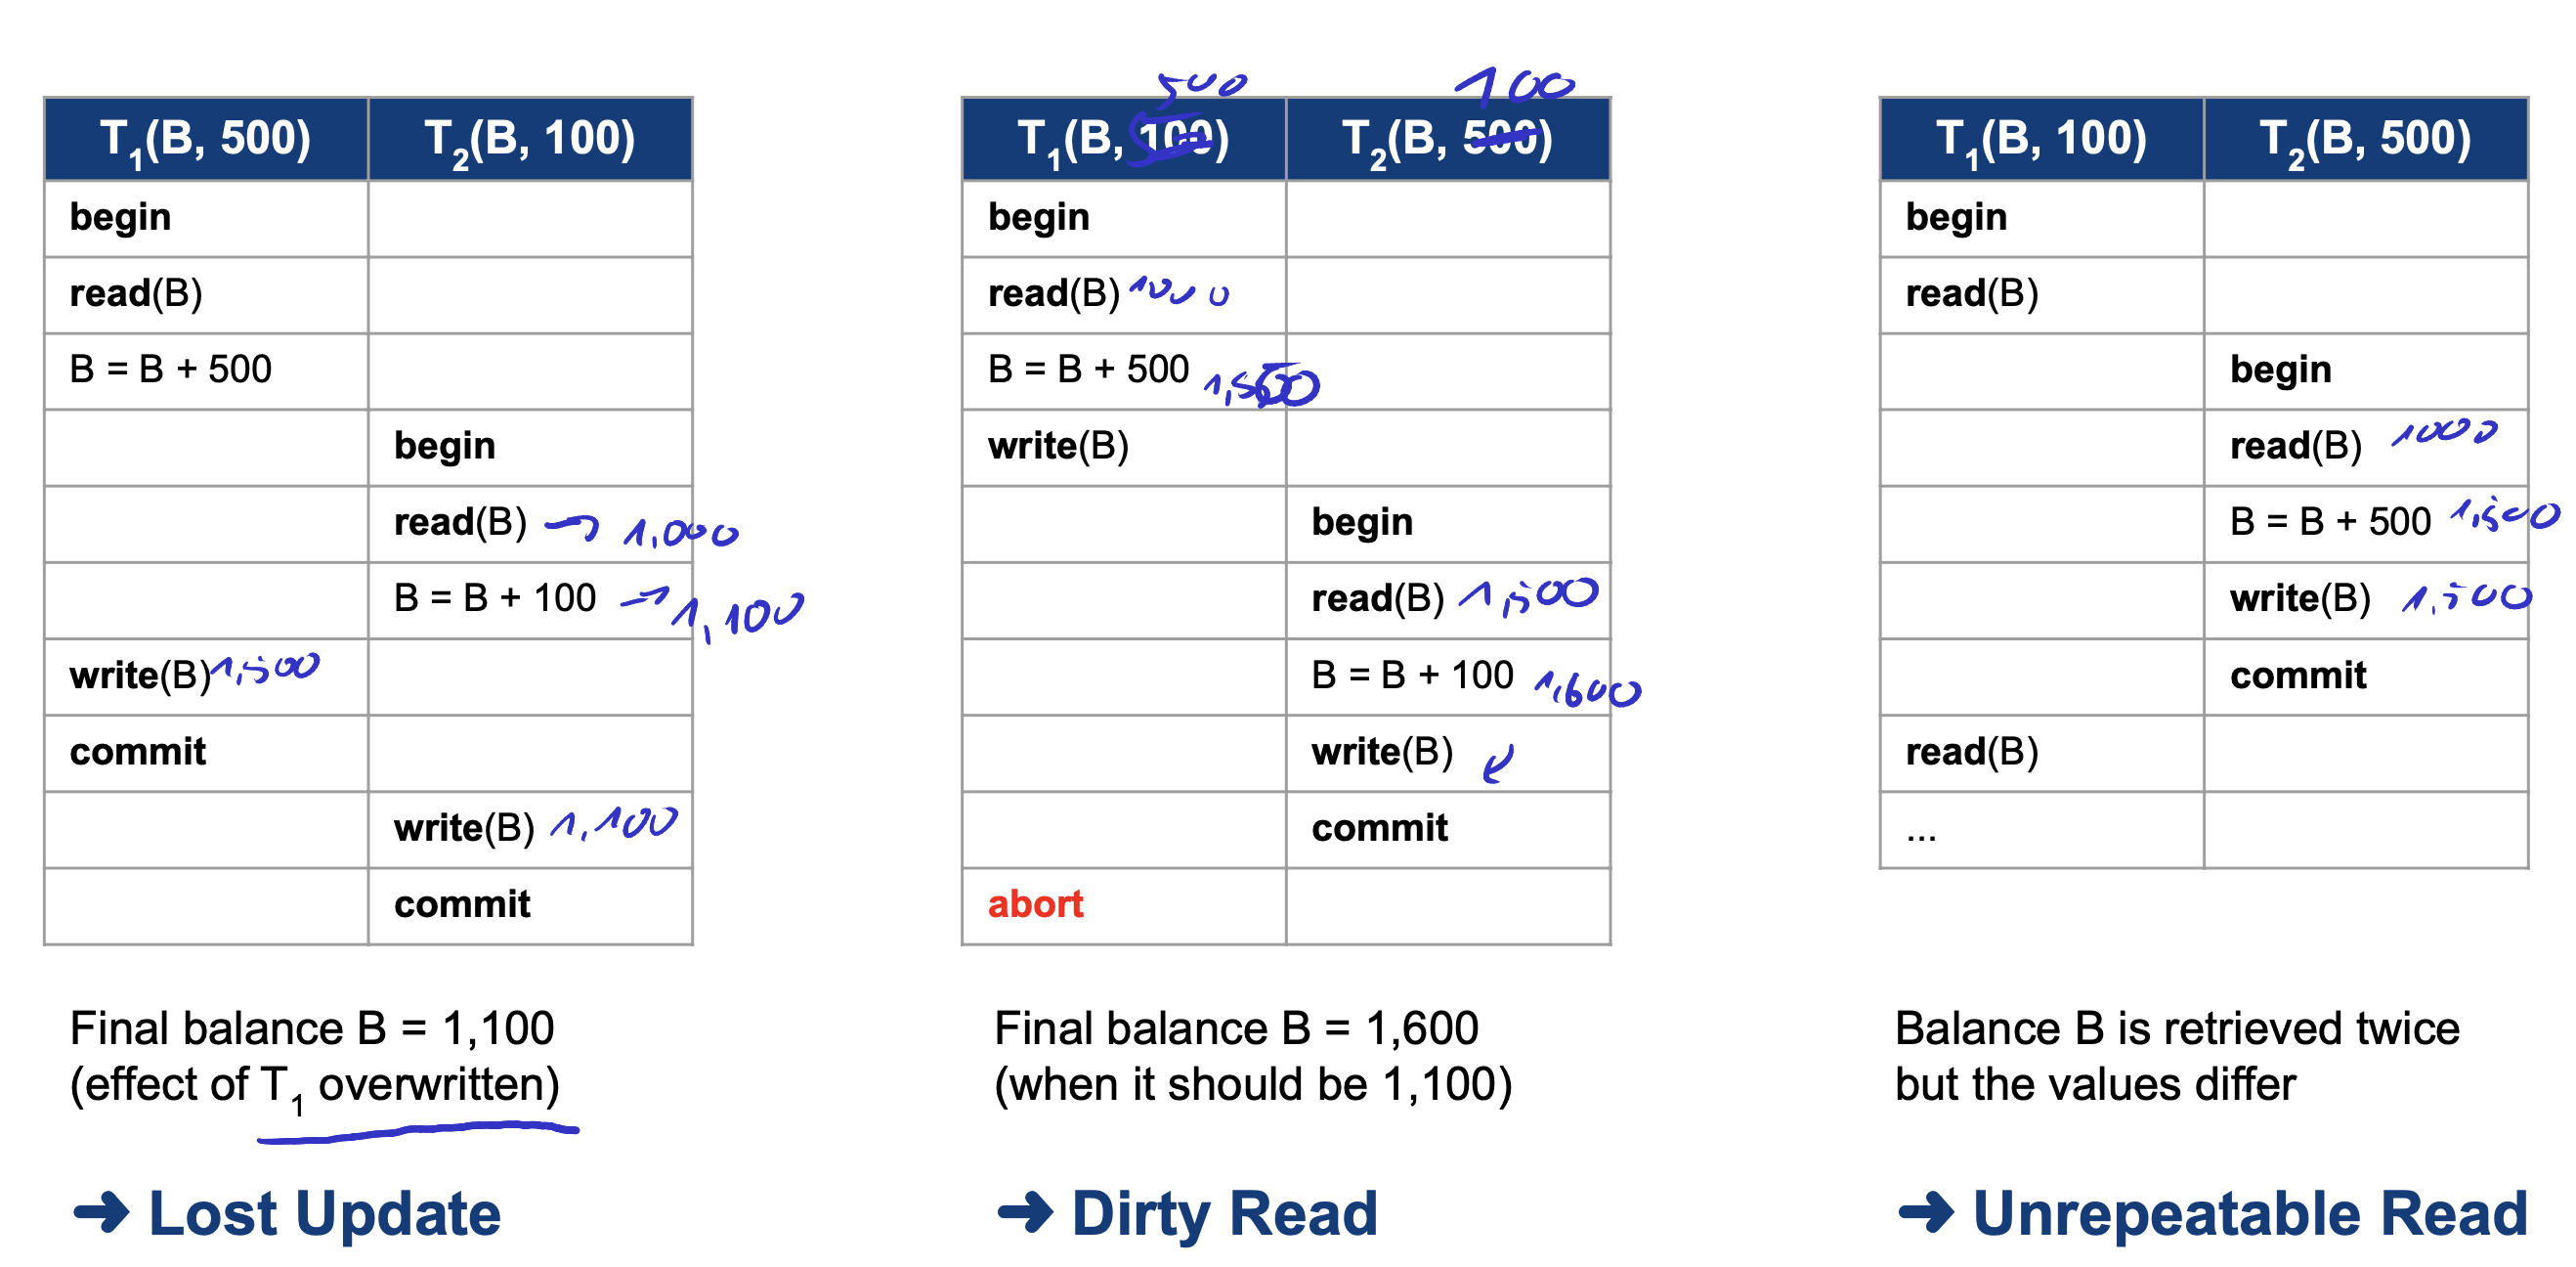
\includegraphics[width=\columnwidth]{L1/concurrent-execution}
    \subsubsection*{Requirements}
      \begin{itemize}[leftmargin=*]
        \item Want serializable transaction execution
          \begin{itemize}[leftmargin=*]
            \item A concurrent execution of a set of transactions is \textbf{serializable} if this execution is equivalent to some serial execution of the same set of instructions
            \item Two executions are equivalent if they have the same effect on the data
          \end{itemize}
        \item Hence, DBMS
          \begin{itemize}[leftmargin=*]
            \item Supports concurrent executions of transactions to optimize performance
            \item Enforces serializability of concurrent executions to ensure integrity of data
          \end{itemize}
      \end{itemize}
  \subsection*{DBMS}
    \begin{itemize}[leftmargin=*]
      \item Is a set of universal and powerful functionalities for data management
      \item Complex, low-level code moved from application logic to DBMS
    \end{itemize}
    \paragraph{Benefits}
      \begin{hlist}
        \item Faster application development
        \item Increased productivity
        \item Higher stability / less errors
      \end{hlist}
    \subsubsection*{Data abstraction} \noindent
      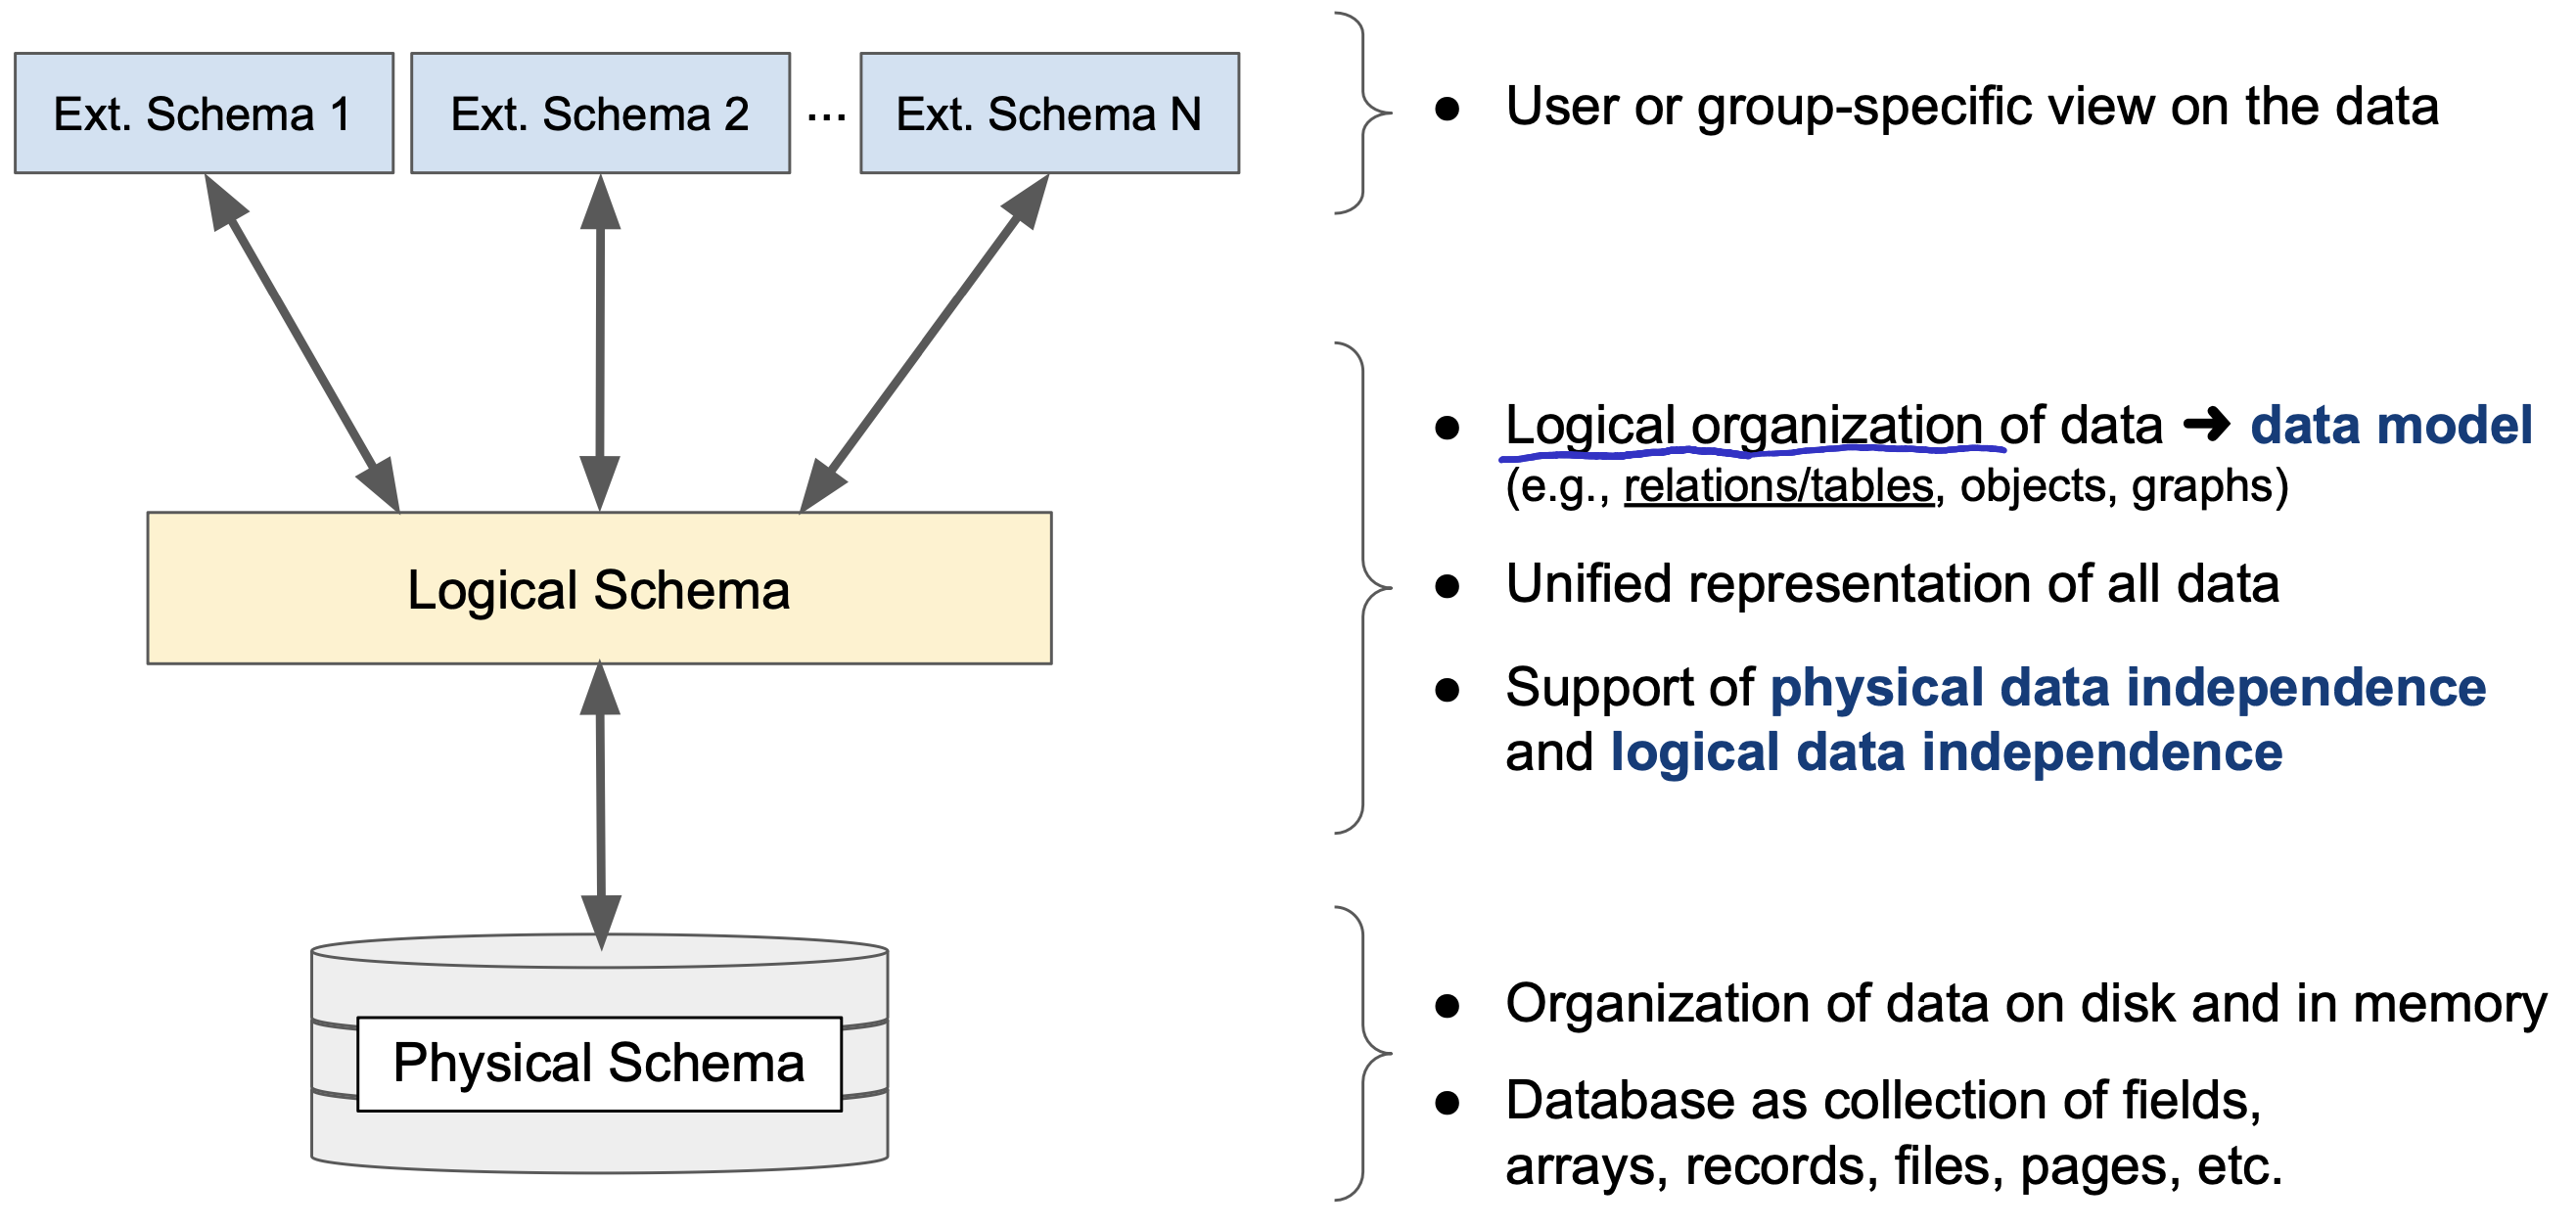
\includegraphics[width=\columnwidth]{L1/data-abstraction}
    \subsubsection*{Data independence} \noindent
      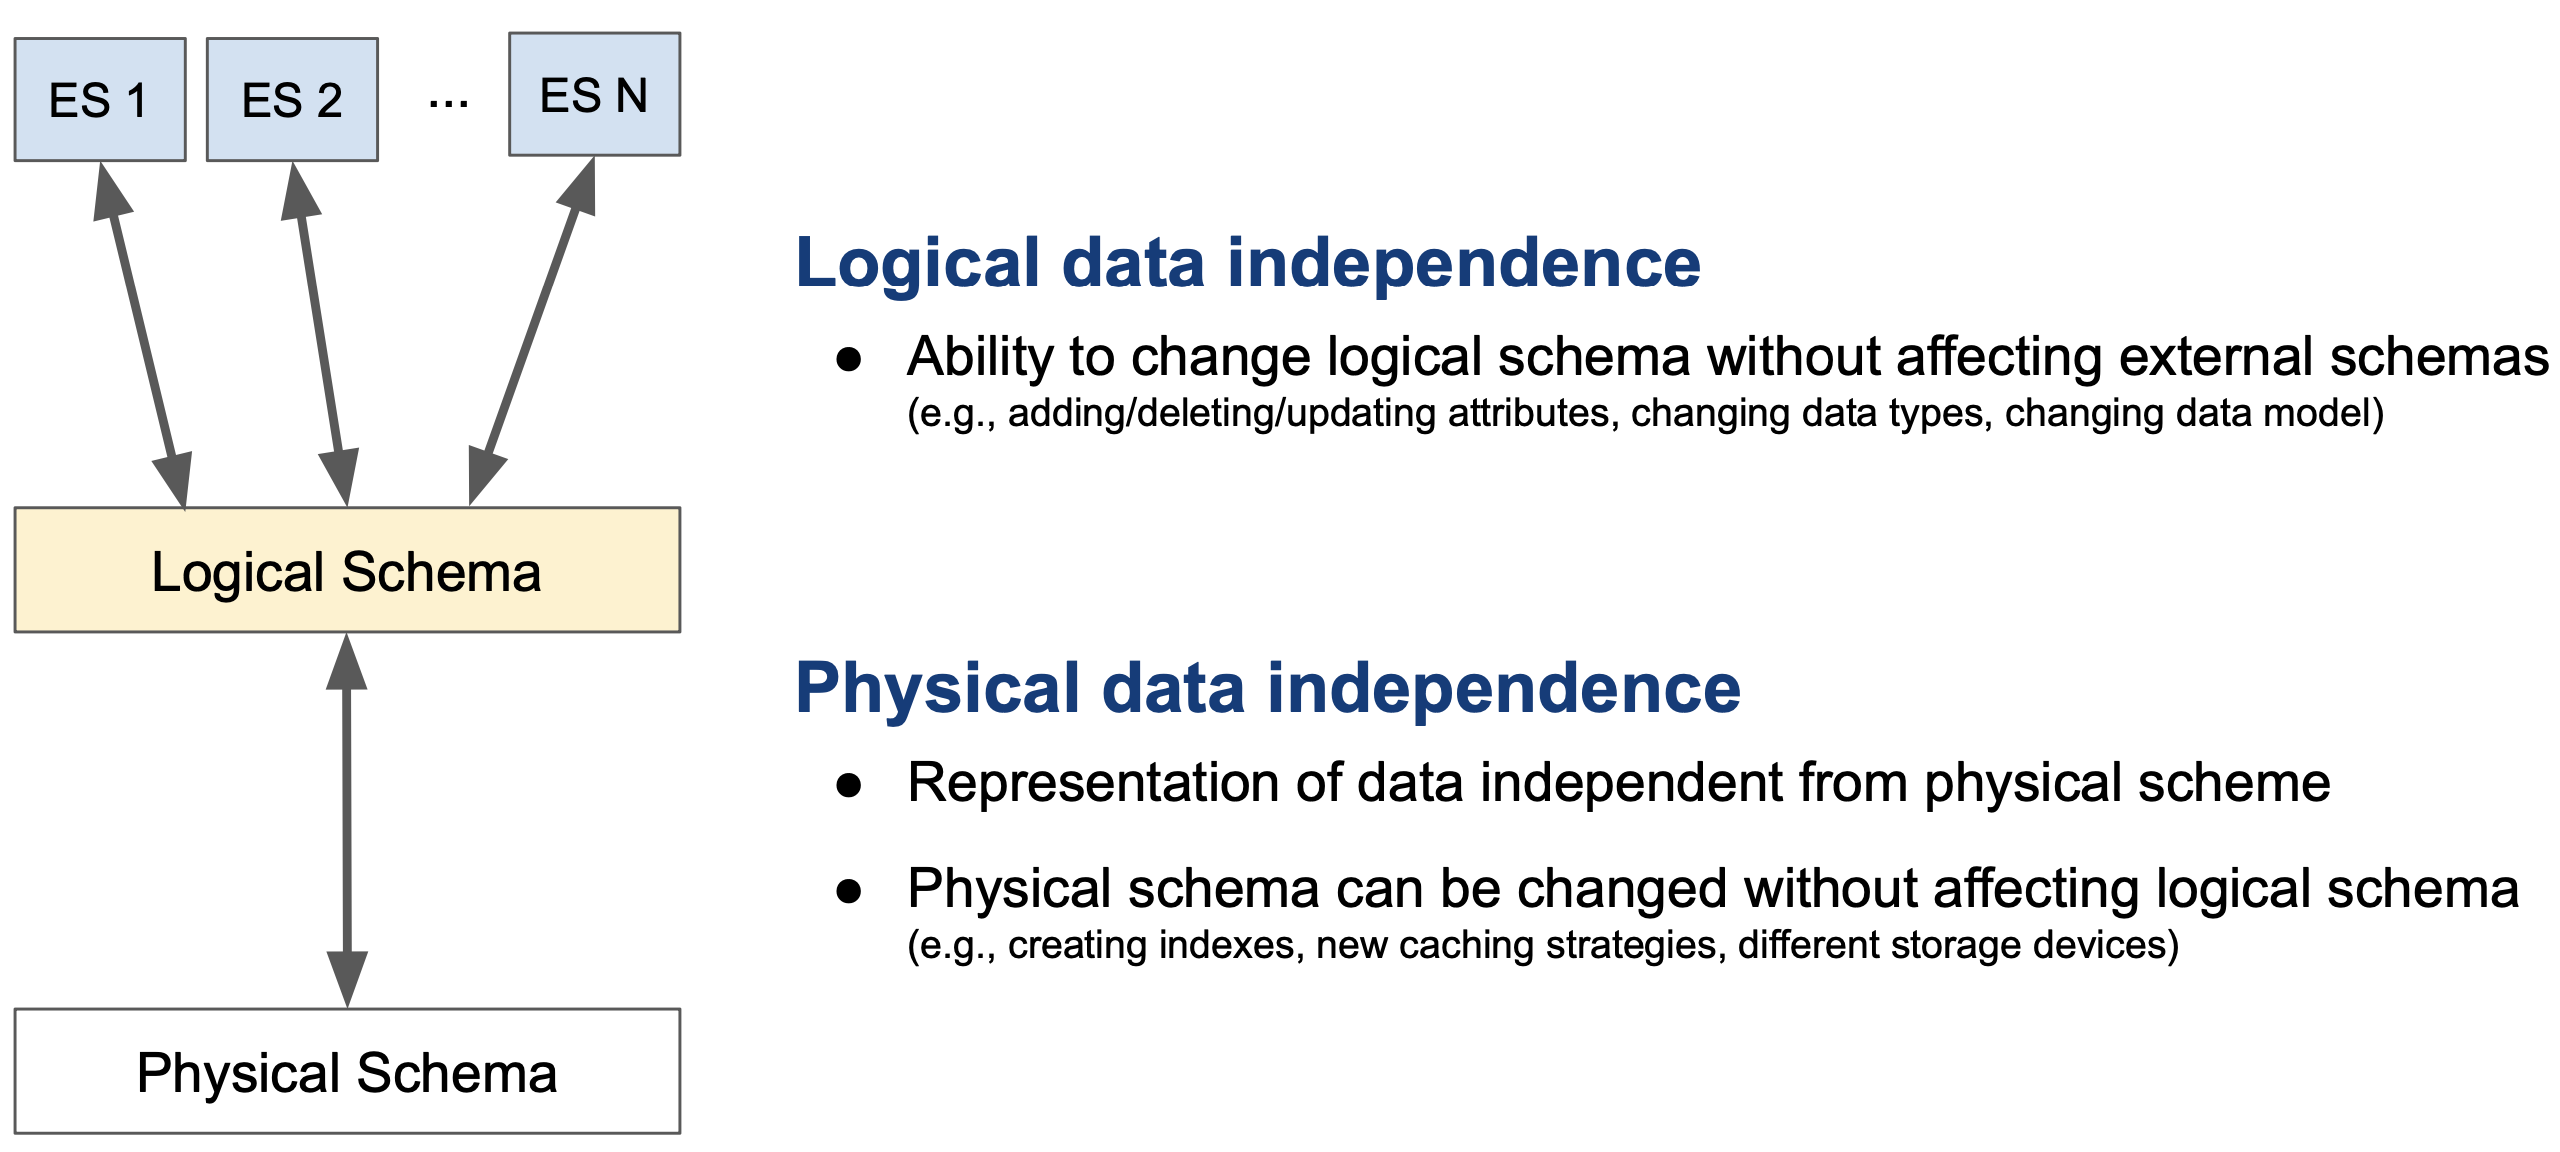
\includegraphics[width=\columnwidth]{L1/data-independence}
    \subsubsection*{Terminology}
      \paragraph{Data model}
        \begin{itemize}[leftmargin=*]
          \item Set of concepts for describing data
          \item Framework to specify structure of a DB
          \item e.g. Relational model, where everything is a table
        \end{itemize}
      \paragraph{Schema}
        Description of structure of a DB, using the concepts provided by data model
      \paragraph{Schema instance}
        Content of a DB at a particular time
  \subsection*{Relational Model}
    \subsubsection*{Terminology}
      \paragraph{Relation}
        \begin{itemize}[leftmargin=*]
          \item Set of tuples (or records)
          \item $R(A_1, A_2, \cdots, A_n)$: relation schema with name $R$, and $n$ attributes $A_1, A_2, \cdots, A_n$
          \item Each instance of schema $R$ is a relation which is a subset of
            \[ \{(a_1, a_2, \cdots, a_n) \;\vert\; a_i \in dom(A_i) \cup \{null\} \} \]
        \end{itemize}
      \paragraph{Relation schema}
        \begin{itemize}[leftmargin=*]
          \item Definition of a relation
          \item Specifies relation name, attributes (columns) and data constraints (e.g. domain constraints)
            \begin{itemize}[leftmargin=*]
              \item Employees (id: \textbf{integer}, name: \textbf{text}, dob: \textbf{date}, salary: \textbf{numeric})
            \end{itemize}
        \end{itemize}
      \paragraph{Domain} Set of atomic values (e.g. integer, numeric, text)
        \begin{itemize}[leftmargin=*]
          \item Domain of attribute $A_i$, $dom(A_i) =$ set of possible values of $A_i$
          \item Each value $v$ of attribute $A_i$: either $v \in dom(A_i)$ or $v =$ \textbf{null}
          \item \textbf{null} - special value indicating the $v$ is not known or not specified
        \end{itemize}
      \paragraph{Relational database schema} Set of relation schemas + data constraints
      \paragraph{Relational database} Collection of tables
      \paragraph{DB vs DBS vs DBMS}
        \[ DBS = DBMS + n \times DB, \quad \text{where } n > 0 \]
  \subsection*{Integrity constraints}
    \begin{itemize}[leftmargin=*]
      \item Condition that restricts what constitutes valid data
      \item 3 main structural integrity constarints of the Relation Model
        \begin{itemize}[leftmargin=*]
          \item 
            \begin{hlist}
              \item Domain constraints
              \item Key constraints
              \item Foreign key (referential integrity) constraints
            \end{hlist}
        \end{itemize}
    \end{itemize}
    \subsubsection*{Domain constraints}
      \begin{itemize}[leftmargin=*]
        \item Data type
        \item NOT NULL / UNIQUE / PRIMARY KEY / FOREIGN KEY / CHECK / DEFAULT
      \end{itemize}
    \subsubsection*{Key constraints}
      \paragraph{Superkey} Subset of attributes that \textbf{uniquely} identifies a tuple in a relation
      \paragraph{Key} Superkey that is also minimal (i.e. no proper subset of the key is a superkey)
      \paragraph{Candidate keys} Set of all possible keys for a relation
      \paragraph{Primary key}
        \begin{itemize}[leftmargin=*]
          \item Chosen candidate key for a relation
          \item Cannot be \textbf{null} (entity integrity constraint)
          \item Underlined in relation schema
            \begin{itemize}[leftmargin=*]
              \item Employees (\underline{id: \textbf{integer}}, name: \textbf{text}, dob: \textbf{date}, salary: \textbf{numeric})
            \end{itemize}
        \end{itemize}
      \paragraph{Prime attribute} Attribute of a primary key (cannot be null)
    \subsubsection*{Foreign key constraints}
      \paragraph{Foreign key}
        \begin{itemize}[leftmargin=*]
          \item Subset of attributes of relation A that refer to the primary key in a relation B
          \item Each foreign key in referencing relation must either
            \begin{itemize}[leftmargin=*]
              \item Appear as primary key in referenced relation, or
              \item Be \textbf{null}
            \end{itemize}
        \end{itemize}
      \paragraph{Properties}
        \begin{itemize}[leftmargin=*]
          \item Specified by DB designer to define what constitutes valid data
          \item Referencing and referenced relation can be the same relation (e.g. each employee has at most one manager)
          \item Relation can be referencing and referenced relation for different relations
        \end{itemize}
    \subsubsection*{Limitations}
      \begin{itemize}[leftmargin=*]
        \item Covers application-independent constraints (e.g. limit domain to valid values)
        \item Does not cover application-dependent constraints derived from deeper semantics of the data
      \end{itemize}
    \subsubsection*{Practical considerations}
      \begin{itemize}[leftmargin=*]
        \item Optional, not mandatory
        \item May affect performance, since checking constraints require additional processing
      \end{itemize}
\section*{Relational Algebra}
  \begin{itemize}[leftmargin=*]
    \item Relations are closed under the Relational Algebra
  \end{itemize}
  \subsection*{Unary operators}
    \subsubsection*{Selection $\sigma_c$}
      \begin{itemize}[leftmargin=*]
        \item For each tuple $t \in R$, $t \in \sigma_c(R) \iff$ selection condition $c$ evaluates to true for tuple $t$.
        \item Input and output have same schema
        \item e.g. Find all projects where Judy is the manager:
          \[ \sigma_{\text{manager=`Judy'}}(\text{Projects}) \]
      \end{itemize}
      \paragraph{Selection condition} is a boolean expression of one of the following forms:
        \vspace{-0.4cm}
        \begin{center}
          \resizebox{\hsize}{!}{%
            \begin{tabular}{ |c|c| }
              \hline
              expression & example \\ \hline
              attribute \textbf{op} constant & $\sigma_{\text{start}=2020}(\text{Projects})$ \\ \hline
              $attr_1$ \textbf{op} $attr_2$ & $\sigma_{\text{start}=\text{end}}(\text{Projects})$ \\ \hline
              $expr_1 \land expr_2$ & $\sigma_{\text{start}=2020 \,\land\, \text{end}=2021}(\text{Projects})$ \\ \hline
              $expr_1 \lor expr_2$ & $\sigma_{\text{start}=2020 \,\lor\, \text{end}=2021}(\text{Projects})$ \\ \hline
              $\neg \, expr$ & $\sigma_{\neg(\text{start}=2020)}(\text{Projects})$ \\ \hline
              $(expr)$ & - \\ \hline
            \end{tabular}
          }
        \end{center}
        where
        \begin{itemize}[leftmargin=*]
          \item \textbf{op} $\in \{ =, <>, <, \leq, \geq, > \}$
          \item Precedence: $(), \textbf{op}, \neg, \land, \lor$
          \item Comparision with \textbf{null} is \textbf{unknown}, arithmetic with \textbf{null} is \textbf{null}
        \end{itemize}
        In boolean expressions, treat unknown as literally unknown. e.g.
        \begin{itemize}[leftmargin=*]
          \item false $\land$ unknown = false
          \item false $\lor$ unknown = unknown
          \item $\neg$ unknown = unknown
          \item true $\land$ unknown = unknown
          \item true $\lor$ unknown = true
        \end{itemize}
    \subsubsection*{Projection $\pi_l$}
      \begin{itemize}[leftmargin=*]
        \item Projects columns of a table specified in list $l$
        \item Order of attributes in $l$ matters
        \item Duplicates are removed, because a relation is a set of tuples
      \end{itemize}
      \paragraph{Example} \mbox{} \\
        \begin{minipage}{0.575 \columnwidth}
          \begin{center}
            Teams \\
            \begin{tabular}{ |c|c|c| }
              \hline
              \textbf{ename} & \textbf{pname} & \textbf{hours} \\ \hline
              Sarah & BigAI & 10 \\ \hline
              Sam & BigAI & 5 \\ \hline
              Sam & BigAI & 3 \\ \hline
            \end{tabular}
          \end{center}
        \end{minipage}
        \hfill
        \begin{minipage}{0.4 \columnwidth}
          \begin{center}
            $\pi_{\text{pname}, \text{ename}}(\text{Teams})$ \\
            \begin{tabular}{ |c|c|c| }
              \hline
              \textbf{pname} & \textbf{ename} \\ \hline
              BigAI & Sarah \\ \hline
              BigAI & Sam \\ \hline
            \end{tabular}
          \end{center}
        \end{minipage}
    \subsubsection*{Renaming $\rho_l$}
      \begin{itemize}[leftmargin=*]
        \item Renames attributes of a relation
      \end{itemize}
      Consider $R(\text{ename, pname, hours})$. Rename ename to name, pname to title. Can either specify
      \begin{itemize}[leftmargin=*]
        \item list of all attr.: $\rho_{(\text{name, title, hours})}(R)$
        \item or list of renames: 
          \[ \rho_{\text{name $\leftarrow$ ename, title $\leftarrow$ pname}}(R) \]
      \end{itemize}
  \subsection*{Set operations} \noindent
    \begin{itemize}[leftmargin=*]
      \item Union, Intersection, Set difference (all obvious)
      \item Note: intersection can be expressed with union and set difference:
        \[ R \cap S = (R \cup S) - ((R-S) \cup (S-R)) \]
      \item The two relations must be union-compatible
    \end{itemize}
    \subsubsection*{Union compatability} \noindent
      Two relations are union-compatible if
      \begin{itemize}[leftmargin=*]
        \item Same number of attributes
        \item Corresponding attributes have same or compatible domains (different attribute names are ok)
      \end{itemize}
      \paragraph{Example}
        The following are union-compatible.
        \begin{itemize}[leftmargin=*]
          \item Employees(name: \textbf{text}, role: \textbf{text}, age: \textbf{integer})
          \item Teams(ename: \textbf{text}, pname: \textbf{text}, hours: \textbf{integer})
        \end{itemize}
    \subsubsection*{Cross product} \noindent
      Forms all possible pairs of tuples from the two relations
  \subsection*{Division operator} \noindent
    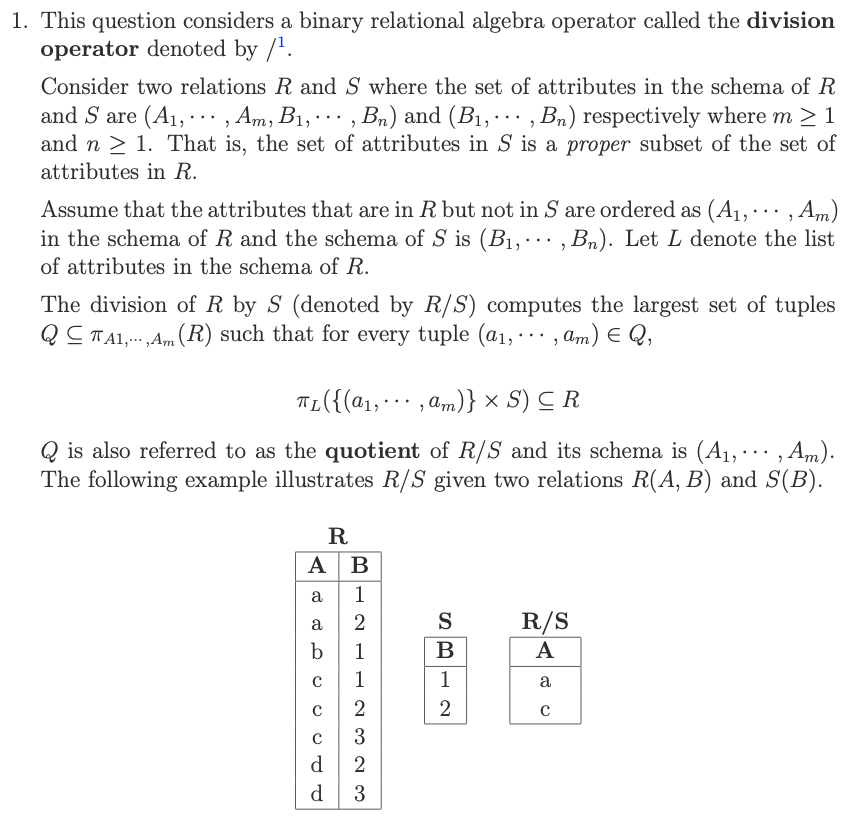
\includegraphics[width=\columnwidth]{division-operator}
  \subsection*{Join operations}
    \begin{itemize}[leftmargin=*]
      \item Combines $\times, \sigma_c, \pi_l$ into a single op
      \item Simple relational algebra expressions
    \end{itemize}
  \subsection*{Inner joins}
    \begin{itemize}[leftmargin=*]
      \item Eliminates tuples that do not satisfy matching criteria (i.e. selection)
      \item Is a selection from cross product
    \end{itemize}
    \subsubsection*{$\theta$-Join} \noindent
      \[ R \Join_\theta S = \sigma_\theta(R \times S) \]
    \subsubsection*{Equi Join} \noindent
      Like $\theta$-Join, but $\theta$ must only involve $=$
    \subsubsection*{Natural Join} \noindent
      Like equi join (i.e. only equality operator), but
      \begin{itemize}[leftmargin=*]
        \item Join is performed over common attributes of $R$ and $S$
        \item If there are no common attributes, acts like a cross product, since selection condition $c$ is vacuously true
        \item Output relation keeps one copy of common attributes
      \end{itemize}
      Formally,
      \[ R \Join S = \pi_l(R \Join_c \rho_{b_i \leftarrow a_i, \cdots, b_k \leftarrow a_k} (S)) \]
      where
      \begin{itemize}[leftmargin=*]
        \item $A = \{a_i, \cdots, a_k\}$ is the set of common attributes of $R$ and $S$
        \item $c = (a_i = b_i) \land \cdots \land (a_k = b_k)$
        \item $l =$ list of (attr. of $R$ + attr. of $S$ not in $A$)
      \end{itemize}
  \subsection*{Outer joins}
    \begin{itemize}[leftmargin=*]
      \item Inner join + dangling tuples
      \item A \textbf{dangling tuple} is a tuple that doesn't satisfy the inner join condition, i.e. foreign key not referenced in the relation.
    \end{itemize}
    \subsubsection*{Steps}
      \begin{itemize}[leftmargin=*]
        \item Perform inner join $M = R \Join_\theta S$
        \item To $M$, add dangling tuples from
          \[
            \begin{cases}
              R & \text{in left outer join} \leftjoin_\theta \\
              S & \text{in right outer join} \rightjoin_\theta \\
              R \;\text{and}\; S & \text{in full outer join} \fulljoin_\theta \\
            \end{cases}
          \]
        \item Pad missing attribute values with \textbf{null}
      \end{itemize}
    \subsubsection*{Formal definitions}
      \begin{itemize}[leftmargin=*]
        \item Set of dangling tuples in $R$, with respect to $R \Join_\theta S$
          \[ \dangle{R \Join_\theta S} \subseteq R \]
        \item $null(R)$ is a $n$-compoennt tuple of \textbf{null} values, where $n$ is the number of attributes in $R$
        \item Left outer join $(R \leftjoin_\theta S)$
          \[ = (R \Join_\theta S) \cup (\dangle{R \Join_\theta S} \times \{\nullrel{S}\}) \]
        \item Right outer join $(R \rightjoin_\theta S)$
          \[ = (R \Join_\theta S) \cup (\{\nullrel{R}\} \times \dangle{S \Join_\theta R}) \]
        \item Full outer join $(R \fulljoin_\theta S)$
      \end{itemize}
      \[
        \begin{aligned}
          &= (R \Join_\theta S) \cup \Big( (\dangle{R \Join_\theta S} \times \{\nullrel{S}\}) \\
          & \cup (\{\nullrel{R}\} \times \dangle{S \Join_\theta R}) \Big)
        \end{aligned}
      \]
    \subsubsection*{Natural outer joins}
      \begin{itemize}[leftmargin=*]
        \item Like natural inner joins
        \item Only equality operator used for condition
        \item Join is performed over common atributes of $R$ and $S$
        \item Output relation keeps one copy of common attributes
      \end{itemize}
  \subsection*{Complex expressions} \noindent
    There are multiple ways to formulate a query to get the same result, e.g.
    \begin{itemize}[leftmargin=*]
      \item Order of joins
      \item Order of selection (before/after join)
      \item Additional projections to minimize intermediate results
    \end{itemize}
  \subsection*{Invalid expressions}
    \begin{itemize}[leftmargin=*]
      \item Attribute no longer available after projection
        \[ \sigma_{\text{role=`dev'}} (\pi_\text{name,age} (Employees)) \]
      \item Attribute no longer available after renaming
        \[ \sigma_{\text{role=`dev'}} (\rho_{\text{position} \leftarrow \text{role}} (Employees)) \]
      \item Incompatible attribute types
        \[ \sigma_{\text{age=role}} (Employees) \]
    \end{itemize}
    \section*{SQL (Define \& Manipulate)}
  \begin{itemize}[leftmargin=*]
    \item Declarative language: focus on what to compute, not on how to compute
    \item Statement Level Interface - app is a mixture of host language statements and SQL statements
    \item Call Level Interface - app is written in host language, SQL statements passed as arguments
  \end{itemize}
  \subsection*{Data types}
    \begin{itemize}[leftmargin=*]
      \item \ic{CAST(x AS NUMERIC)} for typecasting
        \begin{itemize}[leftmargin=*]
          \item Useful to force floating point division
        \end{itemize}
    \end{itemize}
    \begin{center}
      \resizebox{\hsize}{!}{%
        \begin{tabular}{ |c|c| }
          \hline
          \textbf{type} & \textbf{description} \\ \hline
          boolean & logical Boolean (true/false) \\ \hline
          integer & signed 4-byte integer \\ \hline
          float8 & \makecell{double precision floating-point\\number (8 bytes)} \\ \hline
          numeric(p, s) & \makecell{number with $p$ significant\\digits and $s$ decimal places} \\ \hline
          char(n) & fixed-length character string \\ \hline
          varchar(n) & variable-length character string \\ \hline
          text & variable-length character string \\ \hline
          date & calendar date (year, month, day) \\ \hline
          timestamp & date and time \\ \hline
        \end{tabular}
      }
    \end{center}
    Other extended types:
    \begin{itemize}[leftmargin=*]
      \item Document types: XML, JSON
      \item Spatial types: point, line, polygon, circle, box, path
      \item Special types: money/currency, MAC/IP address
      \item User defined types
    \end{itemize}
  \subsection*{Data definition}
    \subsubsection*{Creating tables} \noindent
      Employees (id: \textbf{integer}, name: \textbf{text}, dob: \textbf{date}, salary: \textbf{numeric})
      \begin{lstlisting}
CREATE TABLE Employees(
  id    INTEGER,
  name  VARCHAR(50),
  age   INTEGER,
  role  VARCHAR(50) DEFAULT `sales'
);
      \end{lstlisting}
    \subsection*{Modifying a schema}
      \begin{lstlisting}
-- change data type
ALTER TABLE Projects ALTER COLUMN name TYPE VARCHAR(200);

-- set default value
ALTER TABLE Projects ALTER COLUMN start_year SET DEFAULT 2021;

-- drop default value
ALTER TABLE Projects ALTER COLUMN start_year DROP DEFAULT;

-- add new column with default value
ALTER TABLE Projects ADD COLUMN budget NUMERIC DEFAULT 0.0;
-- drop column from table
ALTER TABLE Projects DROP COLUMN budget;

-- add FK constraint
ALTER TABLE Teams ADD CONSTRAINT eid_fkey FOREIGN KEY (eid) REFERENCES Employees(id);
-- drop FK constraint
ALTER TABLE Teams DROP CONSTRAINT eid_fkey;

-- drop table
DROP TABLE Projects;
DROP TABLE IF EXISTS Projects; -- avoids throwing error if does not exist

-- drop table with dependent objects
DROP TABLE Projects CASCADE; -- deletes Projects and FK constraint
      \end{lstlisting}
  \subsection*{Data manipulation}
    \subsubsection*{Insert data} \noindent
      \begin{lstlisting}
-- Specify all attribute values
INSERT INTO Employees VALUES (101, `Sarah', 25, `dev');
-- Specify selected attribute values
-- role: sales, age: NULL
INSERT INTO Employees (id, name) VALUES (102, `Judy');
      \end{lstlisting}
    \subsubsection*{Deleting data} \noindent
      \begin{lstlisting}
-- Delete all tuples
DELETE FROM Employees;
-- Delete selected tuples
DELETE FROM Employees WHERE role = 'dev';
      \end{lstlisting}
    \subsubsection*{Updating data} \noindent
      \begin{lstlisting}
-- Update with where clause
UPDATE Employees SET age = age+1 WHERE name='Sarah';
-- Set all age to 0
UPDATE Employees SET age = 0;
-- Uppercase ALL strings
UPDATE Employees SET name=UPPER(name), role=UPPER(role);
      \end{lstlisting}
  \subsection*{Handling NULL}
    \begin{itemize}[leftmargin=*]
      \item Comparison with \textbf{null} is unknown
      \item Arithmetic opertaion with \textbf{null} is \textbf{null}
    \end{itemize}
    \subsubsection*{IS (NOT) NULL}
      \begin{itemize}[leftmargin=*]
        \item value is \textbf{null} $\iff$ evaluates to true
        \item \ic{x IS NOT NULL} equivalent to \ic{NOT (x IS NULL)}
      \end{itemize}
    \subsubsection*{IS (NOT) DISTINCT FROM}
      \begin{itemize}[leftmargin=*]
        \item Equivalent to \ic{x <> y} if $x$ and $y$ both non-null
        \item Both null $\implies$ return false
        \item One null $\implies$ return true
      \end{itemize}
  \subsection*{Constraints}
      \begin{itemize}[leftmargin=*]
        \item All constraints can be named or unnamed (unnamed constraints still get named by DBMS)
        \item All column constraints can be specified as table constraints (except not null)
        \item Table constraints referring to a single column can be specified as column constraint
        \item Column and table constraints can be combined, e.g.
      \end{itemize}
        \begin{lstlisting}
CREATE TABLE Employees (
  -- id specified twice
  id    INTEGER NOT NULL,
  name  VARCHAR(50),
        UNIQUE(id)
);
        \end{lstlisting}
    \subsubsection*{Not-null constraints}
      \begin{itemize}[leftmargin=*]
        \item Violation: $\exists t \in$ Employees where \ic{t.id IS NOT NULL} evaluates to false
      \end{itemize}
      \begin{lstlisting}
CREATE TABLE Employees(
  -- unnamed (name assigned by DBMS)
  id    INTEGER NOT NULL,
  -- named (easier bookkeeping)
  name  VARCHAR(50) CONSTRAINT nn_name NOT NULL
);
      \end{lstlisting}
    \subsubsection*{Unique constraints}
      \begin{itemize}[leftmargin=*]
        \item Violation: For any two tuples $x, y \in$ Teams,
          \ic{(x.id <> y.id)} or \ic{(x.name <> y.name)} evaluates to false
        \item Since \ic{(null <> null)} evaluates to unknown, the tuples \ic{(101, null)} and \ic{(101, null)} are considered unique
        \item Unique constraint involving multiple attributes is specified using table constraints
      \end{itemize}
      \begin{lstlisting}
CREATE TABLE Employees (
  -- column constraint
  id INTEGER UNIQUE,
  name VARCHAR(50),
  -- table constraint
  UNIQUE(id),         -- single attribute
  UNIQUE(id, name),   -- multi attribute
  CONSTRAINT unique_id UNIQUE(id)   -- named
);
      \end{lstlisting}
    \subsubsection*{PK constraints}
      \begin{itemize}[leftmargin=*]
        \item \ic{PRIMARY KEY} and \ic{UNIQUE NOT NULL} have the same effect
        \item Only 1 \ic{PRIMARY KEY}, but can have multiple \ic{UNIQUE NOT NULL}
      \end{itemize}
      \begin{lstlisting}
CREATE TABLE Employees (
  -- These 2 statements have the same effect
  id    INTEGER PRIMARY KEY,
  id    INTEGER UNIQUE NOT NULL,
  --
  name  VARCHAR(50),
        PRIMARY KEY (id, name) -- multiple attributes
);
      \end{lstlisting}
    \subsubsection*{FK constraints} \noindent
      The foreign key must either
      \begin{itemize}[leftmargin=*]
        \item exist in the other table, or
        \item contain NULL in at least one of its attributes
      \end{itemize}
      \begin{lstlisting}
CREATE TABLE Employees (
  id      INTEGER PRIMARY KEY,
  name    VARCHAR(50),
  age     INTEGER
);
CREATE TABLE Projects (
  name        VARCHAR(50) PRIMARY KEY,
  start_year  INTEGER,
  end_year    INTEGER
);
CREATE TABLE Teams (
  eid     INTEGER,       -- eid -> Employee.name
  pname   VARCHAR(100),  -- pid -> Project.name
  hours   INTEGER,
  PRIMARY KEY (ename, pname),
  FOREIGN KEY (eid) REFERENCES Employees (id),
  FOREIGN KEY (pname) REFERENCES Projects (name)
);
      \end{lstlisting}
    \subsubsection*{FK constraints ON action}
      \begin{itemize}[leftmargin=*]
        \item Specify action in case a FK constraint is violated
        \item \ic{ON DELETE/UPDATE <action>}
        \item Both specifications are optional
      \end{itemize}
      \vspace{-0.5cm}
      \begin{center}
        \begin{tabular}{ |c|c| }
          \hline
          \textbf{case} & \textbf{action} \\ \hline
          \makecell{NO ACTION\\(default)} & \makecell{rejects delete/update\\if it violates constraint} \\ \hline
          RESTRICT & \makecell{similar to NO ACTION, but check\\of constraint cannot be \textbf{deferred}} \\ \hline
          CASCADE & \makecell{propagates delete/update\\to referencing tuples\\(can significantly affect performance)} \\ \hline
          SET DEFAULT & \makecell{updates FKs of referencing tuples to\\some default value (default value must\\be a PK in referenced table)} \\ \hline
          SET NULL & \makecell{updates FKs of referencing tuples\\to null (corresponding column must\\be allowed to contain null values)} \\ \hline
        \end{tabular}
      \end{center}
      \begin{lstlisting}
CREATE TABLE Teams (
  eid     INTEGER,
  pname   VARCHAR(100),
  hours   INTEGER,
  PRIMARY KEY (ename, pname),
  FOREIGN KEY (eid) REFERENCES Employees (id) ON DELETE <action> ON UPDATE <action>,
  FOREIGN KEY (pname) REFERENCES Projects (name) ON DELETE <action> ON UPDATE <action>
);
      \end{lstlisting}
    \subsubsection*{Check constraints}
      \begin{itemize}[leftmargin=*]
        \item Specify that column values must satisfy a Boolean expression
        \item Scope: one table, single row
      \end{itemize}
      \begin{lstlisting}
-- column constraint
CREATE TABLE Teams (
  eid     INTEGER PRIMARY KEY,
  pname   VARCHAR(100),
  -- unnamed
  hours   INTEGER check (hours > 0),
  -- named
  hours   INTEGER constraint positive_hours check (hours > 0)
);

-- table constraint
CREATE TABLE Projects (
  name          VARCHAR(50) PRIMARY KEY,
  start_year    INTEGER,
  end_year      INTEGER,
  CHECK (start_year <= end_year)
);
      \end{lstlisting}
      Can be complex Boolean expressions
      \begin{lstlisting}
CREATE TABLE Teams (
  eid     INTEGER PRIMARY KEY,
  pname   VARCHAR(100),
  hours   INTEGER,
  CHECK (
    (pname = `CoreOS' AND hours >= 30)
    OR
    (pname <> `CoreOS' AND hours >= 0)
  )
);
      \end{lstlisting}
  \subsection*{Deferrable constraints}
    \begin{itemize}[leftmargin=*]
      \item Default behavior for constraints: check immediately at the end of SQL statement execution, even for transaction with multiple SQL statements
        \begin{itemize}[leftmargin=*]
          \item Violation causes statement to be rolled back
        \end{itemize}
    \end{itemize}
    \subsubsection*{Deferrable constraints}
      \begin{itemize}[leftmargin=*]
        \item Check can be deferred for some constraints to the end of a transaction
        \item Allows violation of constraints temporarily within the scope of a transaction
        \item Constraint still needs to be resolved at the end of the transaction
        \item Can be used for \ic{UNIQUE}, \ic{PRIMARY KEY}, \ic{FOREIGN KEY}
      \end{itemize}
      \paragraph{Benefits}
        \begin{itemize}[leftmargin=*]
          \item No need to care about order of SQL statements within a transaction
          \item Allows for cyclic FK constraints
          \item Performance boost when constraint checks are bottleneck
        \end{itemize}
      \paragraph{Downsides}
        \begin{itemize}[leftmargin=*]
          \item Difficult to troubleshoot
          \item Data definition no longer unambiguous
          \item Performance penalty when performing queries
        \end{itemize}
\section*{ER model}
  \subsection*{Entity} \noindent
    \begin{itemize}[leftmargin=*]
      \item Objects that are distinguishable from other objects
      \item \textbf{Entity set:} Collection of entities of the same type
    \end{itemize}
  \subsection*{Attribute} \noindent
    \begin{itemize}[leftmargin=*]
      \item Specific information describing an entity
      \item \textbf{Key attribute(s)} uniquely identifies each entity
      \item \textbf{Composite attribute} composed of multiple other attributes
      \item \textbf{Multivalued attribute} may consist of more than one value for a given entity
      \item \textbf{Derived attribute} derived from other attributes
    \end{itemize}
    \begin{center}
      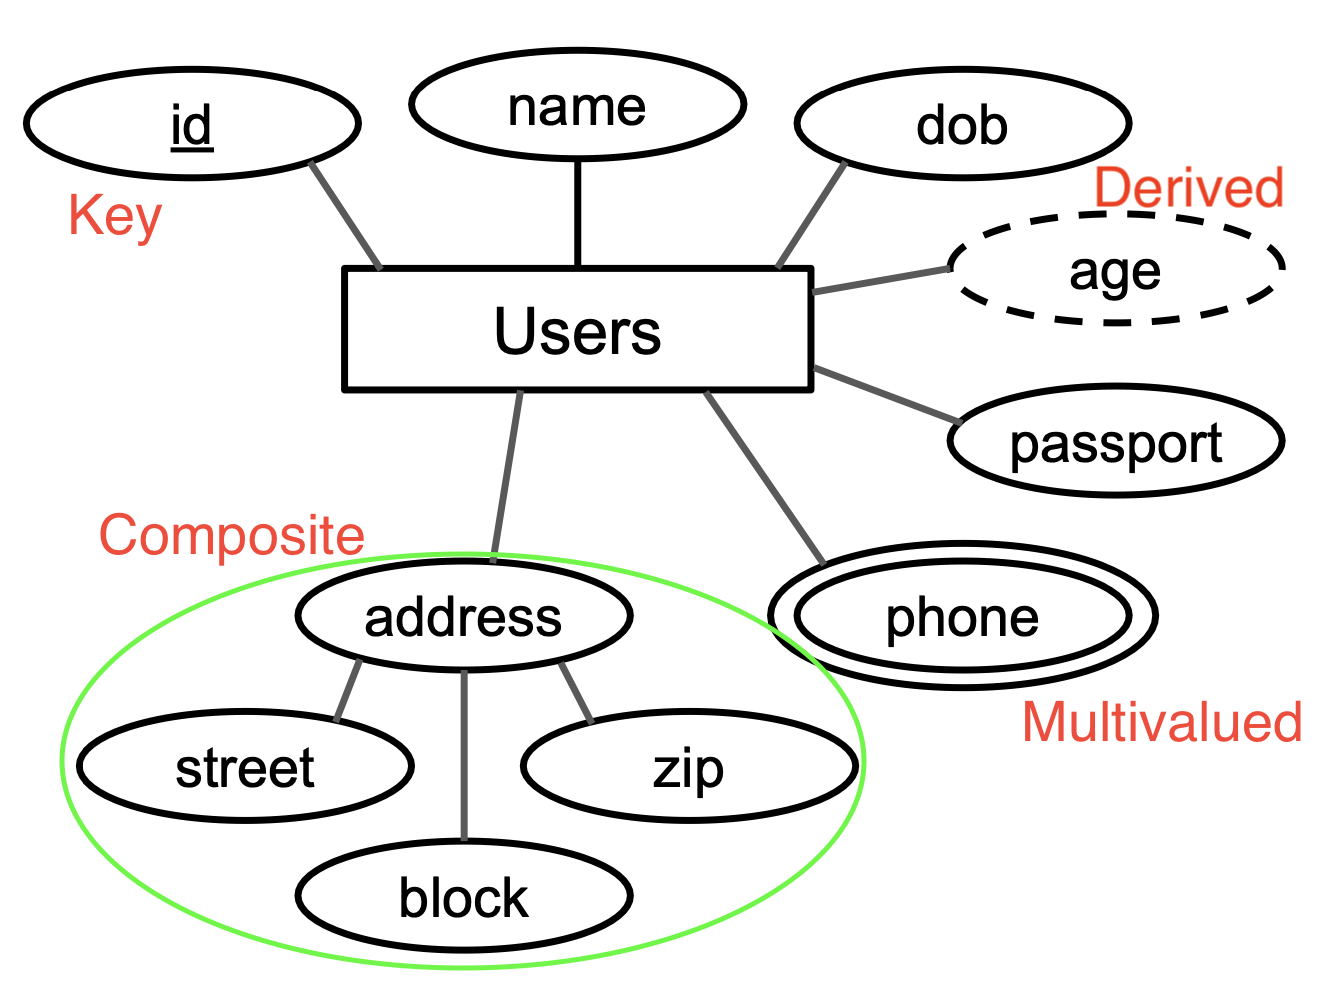
\includegraphics[width=0.5\columnwidth]{L4/attributes}
    \end{center}
  \subsection*{Relationship} \noindent
    Association among two or more entities
    \subsubsection*{Relationship set} \noindent
      \begin{itemize}[leftmargin=*]
        \item Collection of relationships of the same type
        \item Can have their own attributes that further describe the relationship
        \item $Key(E_i)$ is the attributes of the selected key of entity set $E_i$
      \end{itemize}
      \paragraph{Role}
        \begin{itemize}[leftmargin=*]
          \item Describes an entity set's participation in a relationship
          \item Explicit role label only in case of ambiguities (e.g. same entity set participates in same relationship more than once)
        \end{itemize}
      \paragraph{Degree}
        \begin{itemize}[leftmargin=*]
          \item An $n$-ary relationship set involves $n$ entity roles, where $n$ is the degree of the relationship set
          \item Typically binary or ternary
        \end{itemize}
      \begin{minipage}{.5 \columnwidth}
        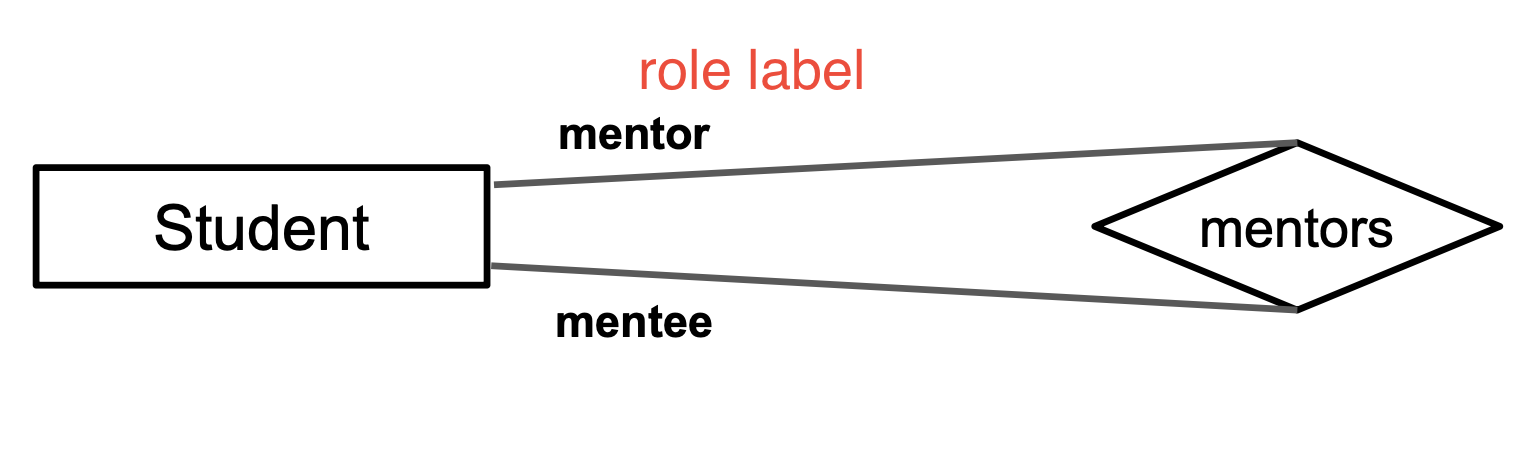
\includegraphics[width=\columnwidth]{L4/role}
      \end{minipage}
      \begin{minipage}{.475 \columnwidth}
        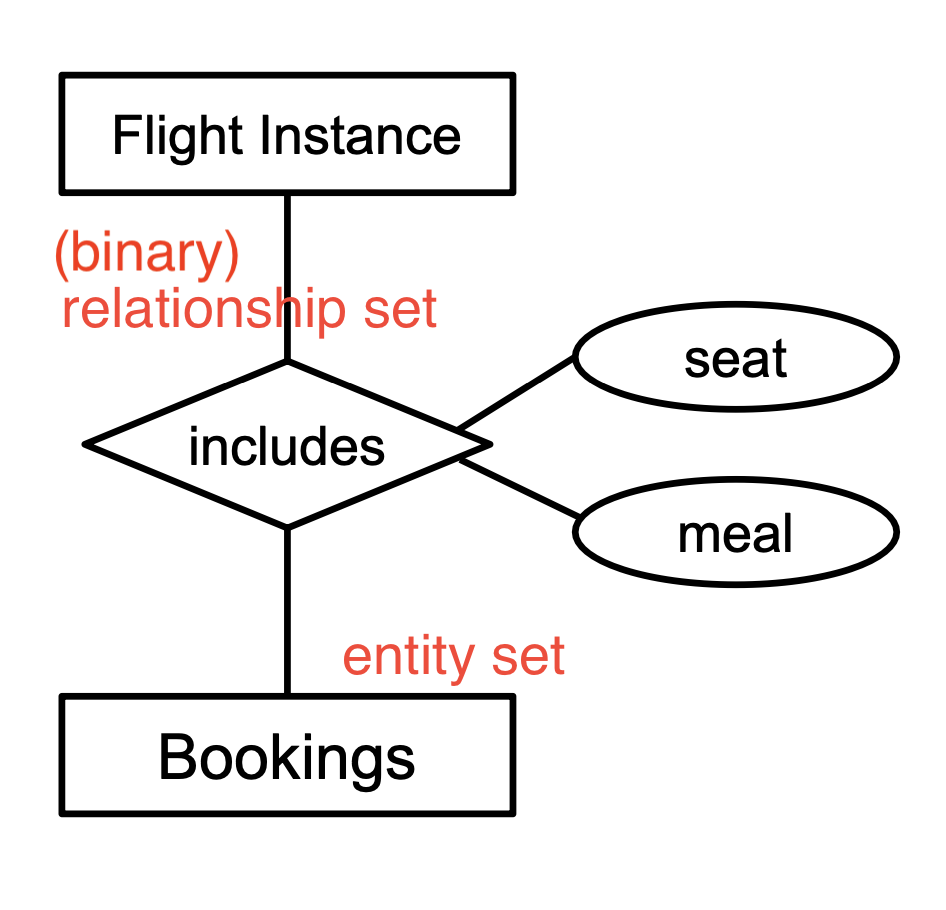
\includegraphics[width=\columnwidth]{L4/relationship-set}
      \end{minipage}
  \subsection*{Cardinality constraints}
    \begin{itemize}[leftmargin=*]
      \item \textbf{Upper bound} for entity's participation
    \end{itemize}
    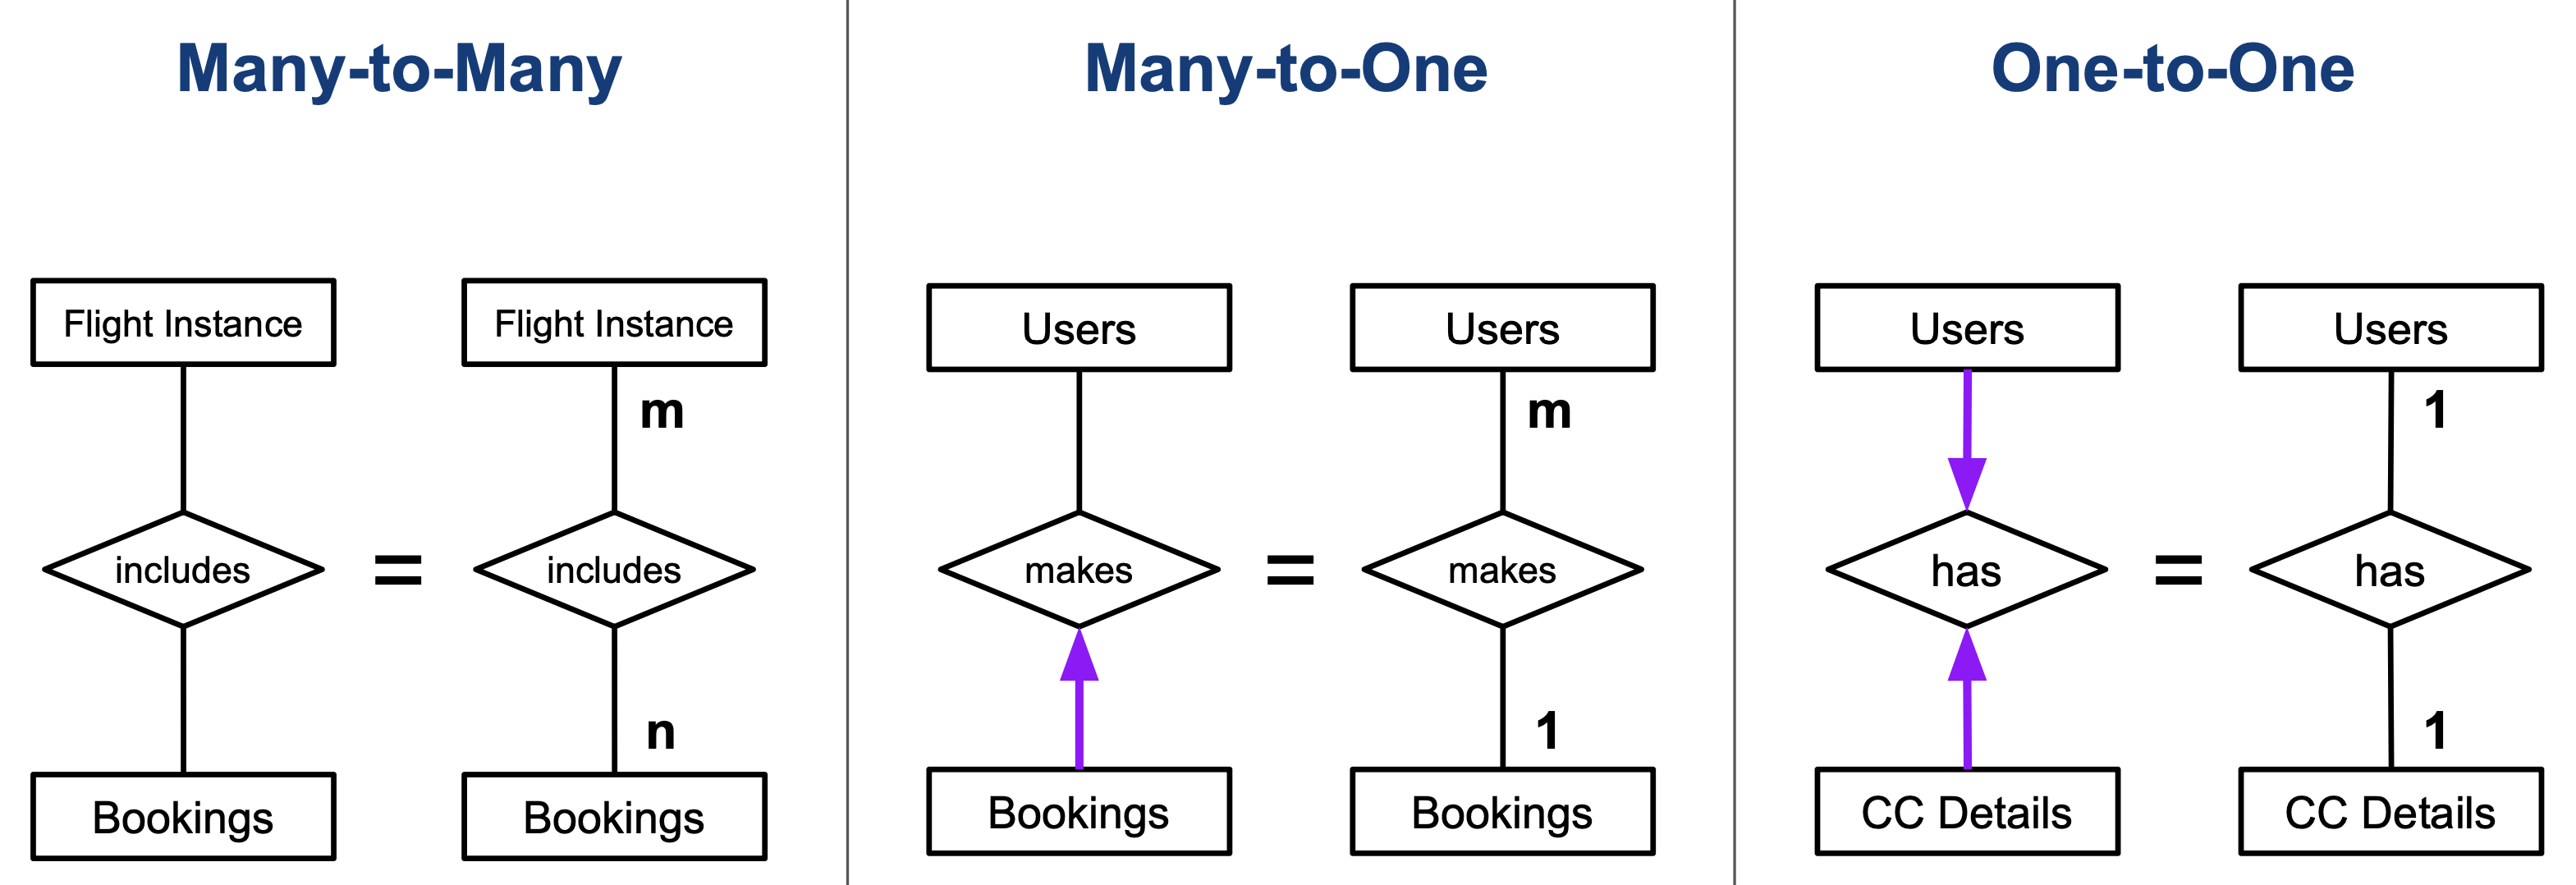
\includegraphics[width=\columnwidth]{L4/cardinality}
  \subsection*{Participation constraints}
    \begin{itemize}[leftmargin=*]
      \item \textbf{Lower bound} for entity's participation
      \item Partial (default): participation not mandatory
      \item Total: mandatory (at least 1)
    \end{itemize}
    \begin{minipage}{.475 \columnwidth}
      \begin{center}
        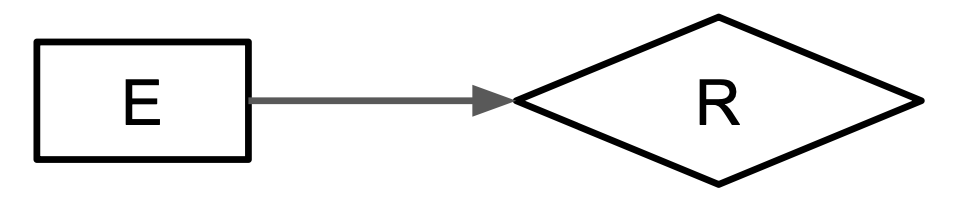
\includegraphics[width=\columnwidth]{L4/participation/at-most-one}
        At most one \\
        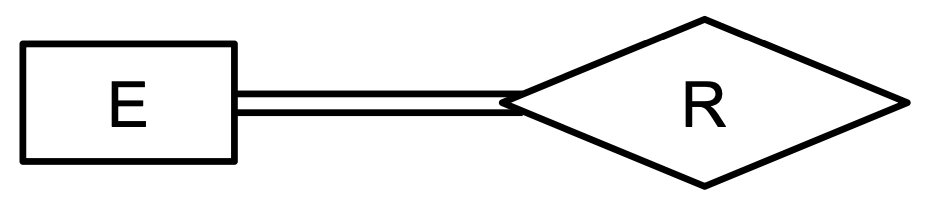
\includegraphics[width=\columnwidth]{L4/participation/at-least-one}
        At least one \\
      \end{center}
    \end{minipage}
    \begin{minipage}{.475 \columnwidth}
      \begin{center}
        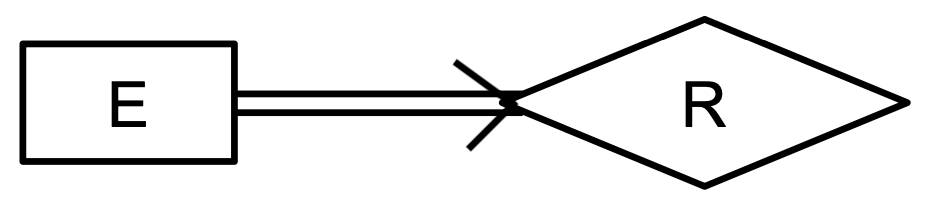
\includegraphics[width=\columnwidth]{L4/participation/exactly-one}
        Exactly one \\
      \end{center}
    \end{minipage}
    \subsubsection*{Alternative} \noindent
      \begin{center}
        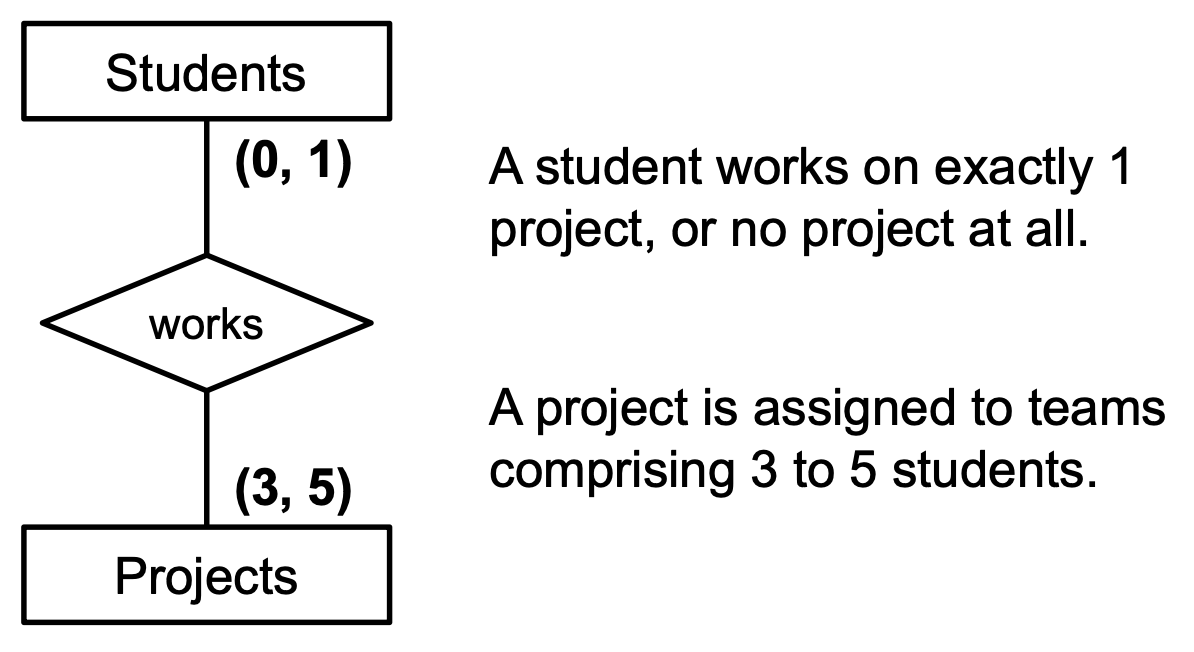
\includegraphics[width=0.5\columnwidth]{L4/participation/min-max}
      \end{center}
    \subsubsection*{Implementation}
      \paragraph{Many-to-Many} Represent relationship set with a table
      \paragraph{Many-to-One}
        \begin{enumerate}[leftmargin=*]
          \item Represent relationship set with a table
          \item Combine relationship set and total participiation entity set into one table
        \end{enumerate}
      \paragraph{One-to-One}
        \begin{enumerate}[leftmargin=*]
          \item Represent relationship set with a table
          \item Combine relationship set and either entity set into one table
        \end{enumerate}
  \subsection*{Dependency constraints}
    \subsubsection*{Weak entity sets}
      \begin{itemize}[leftmargin=*]
        \item Entity set that does not have its own key
        \item Can only be uniquely identified by considering primary key of owner entity
        \item Existence depends on existence of owner entity
      \end{itemize}
      \paragraph{Partial key}
        \begin{itemize}[leftmargin=*]
          \item Set of attributes of weak entity set that uniquely identifies a weak entity, for a given owner entity
        \end{itemize}
      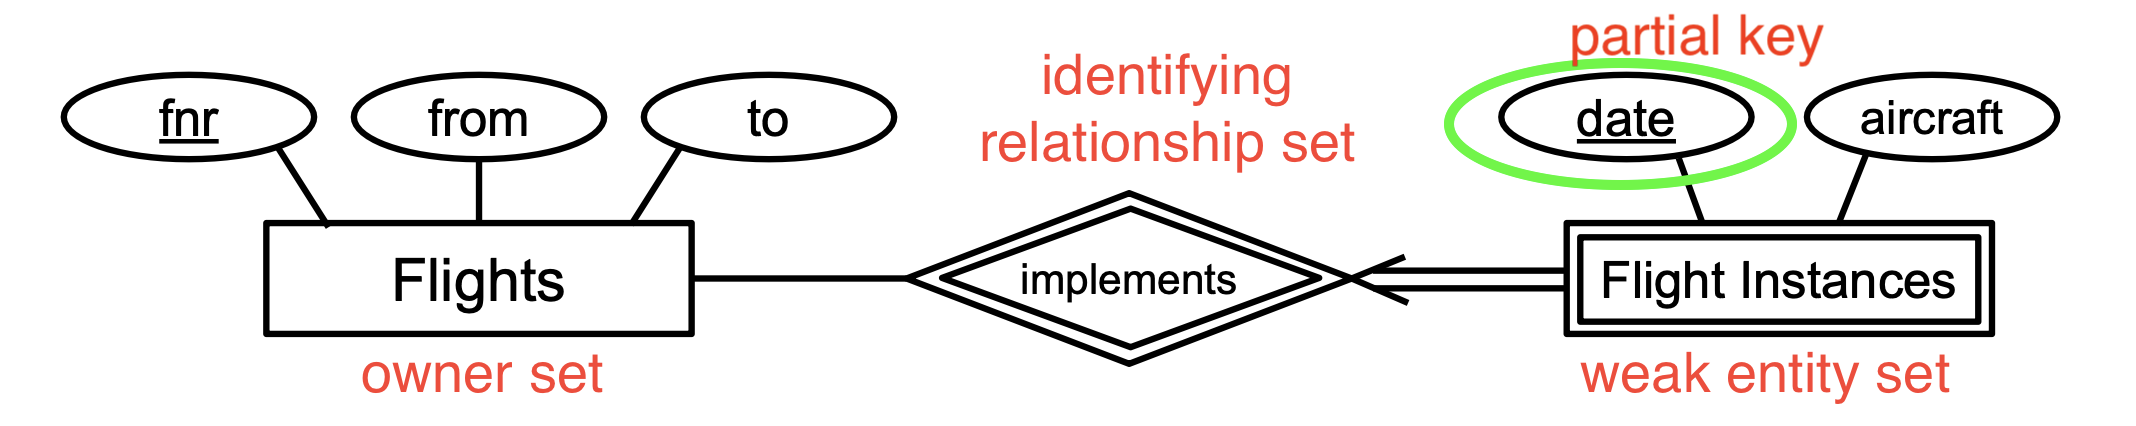
\includegraphics[width=\columnwidth]{L4/weak-entity}
      \paragraph{Requirements}
        \begin{itemize}[leftmargin=*]
          \item Many-to-one relationship from weak entity set to owner entity set
          \item Weak entity set must have total participation in identifying relationship
        \end{itemize}
  \subsection*{Relational mapping}
    \begin{itemize}[leftmargin=*]
      \item Entity set $\rightarrow$ table
      \item Composite/multivalued attributes:
        \begin{enumerate}[leftmargin=*]
          \item Convert to single-valued attributes
          \item Additional table with FK constraint
          \item Convert to a single-valued attribute (e.g. comma separated string)
        \end{enumerate}
    \end{itemize}
  \subsection*{ISA Hierarchies}
    \begin{itemize}[leftmargin=*]
      \item ``Is a" relationship - used to model generalization/specialization of entity sets
    \end{itemize}
    \subsubsection*{Constraints}
      \paragraph{Overlap} Can a superclass entity belong to multiple subclasses?
      \paragraph{Covering} Does a superclass entity have to belong to a subclass?
    \begin{minipage}{.475 \columnwidth}
      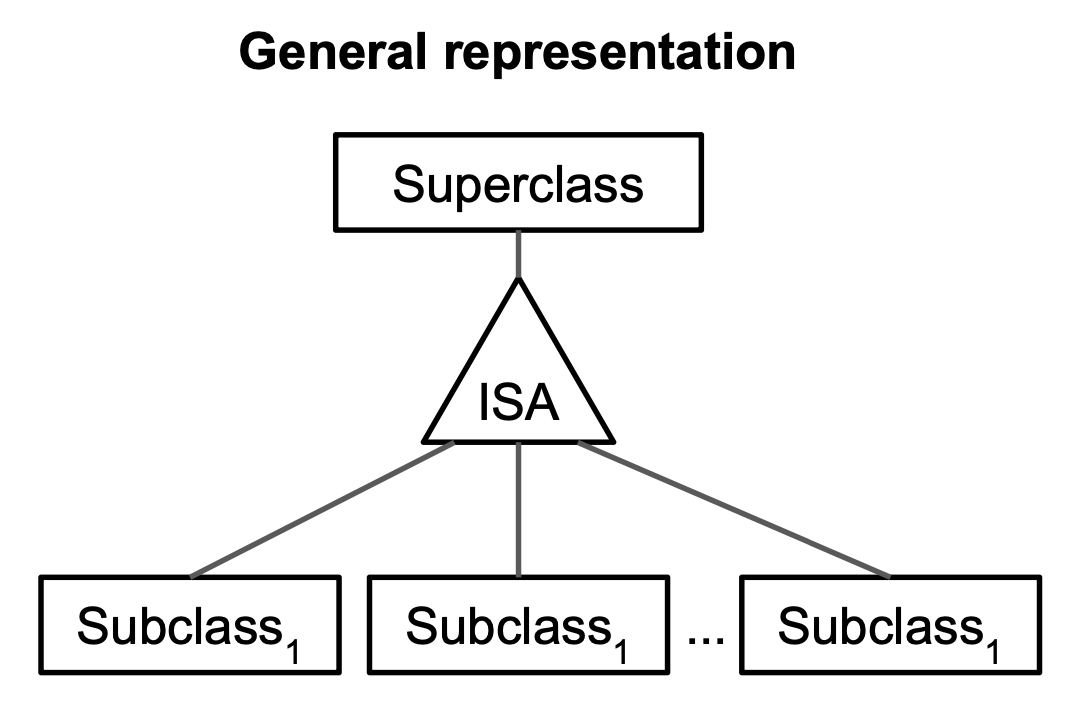
\includegraphics[width=\columnwidth]{L4/is-a}
    \end{minipage}
    \begin{minipage}{.5 \columnwidth}
      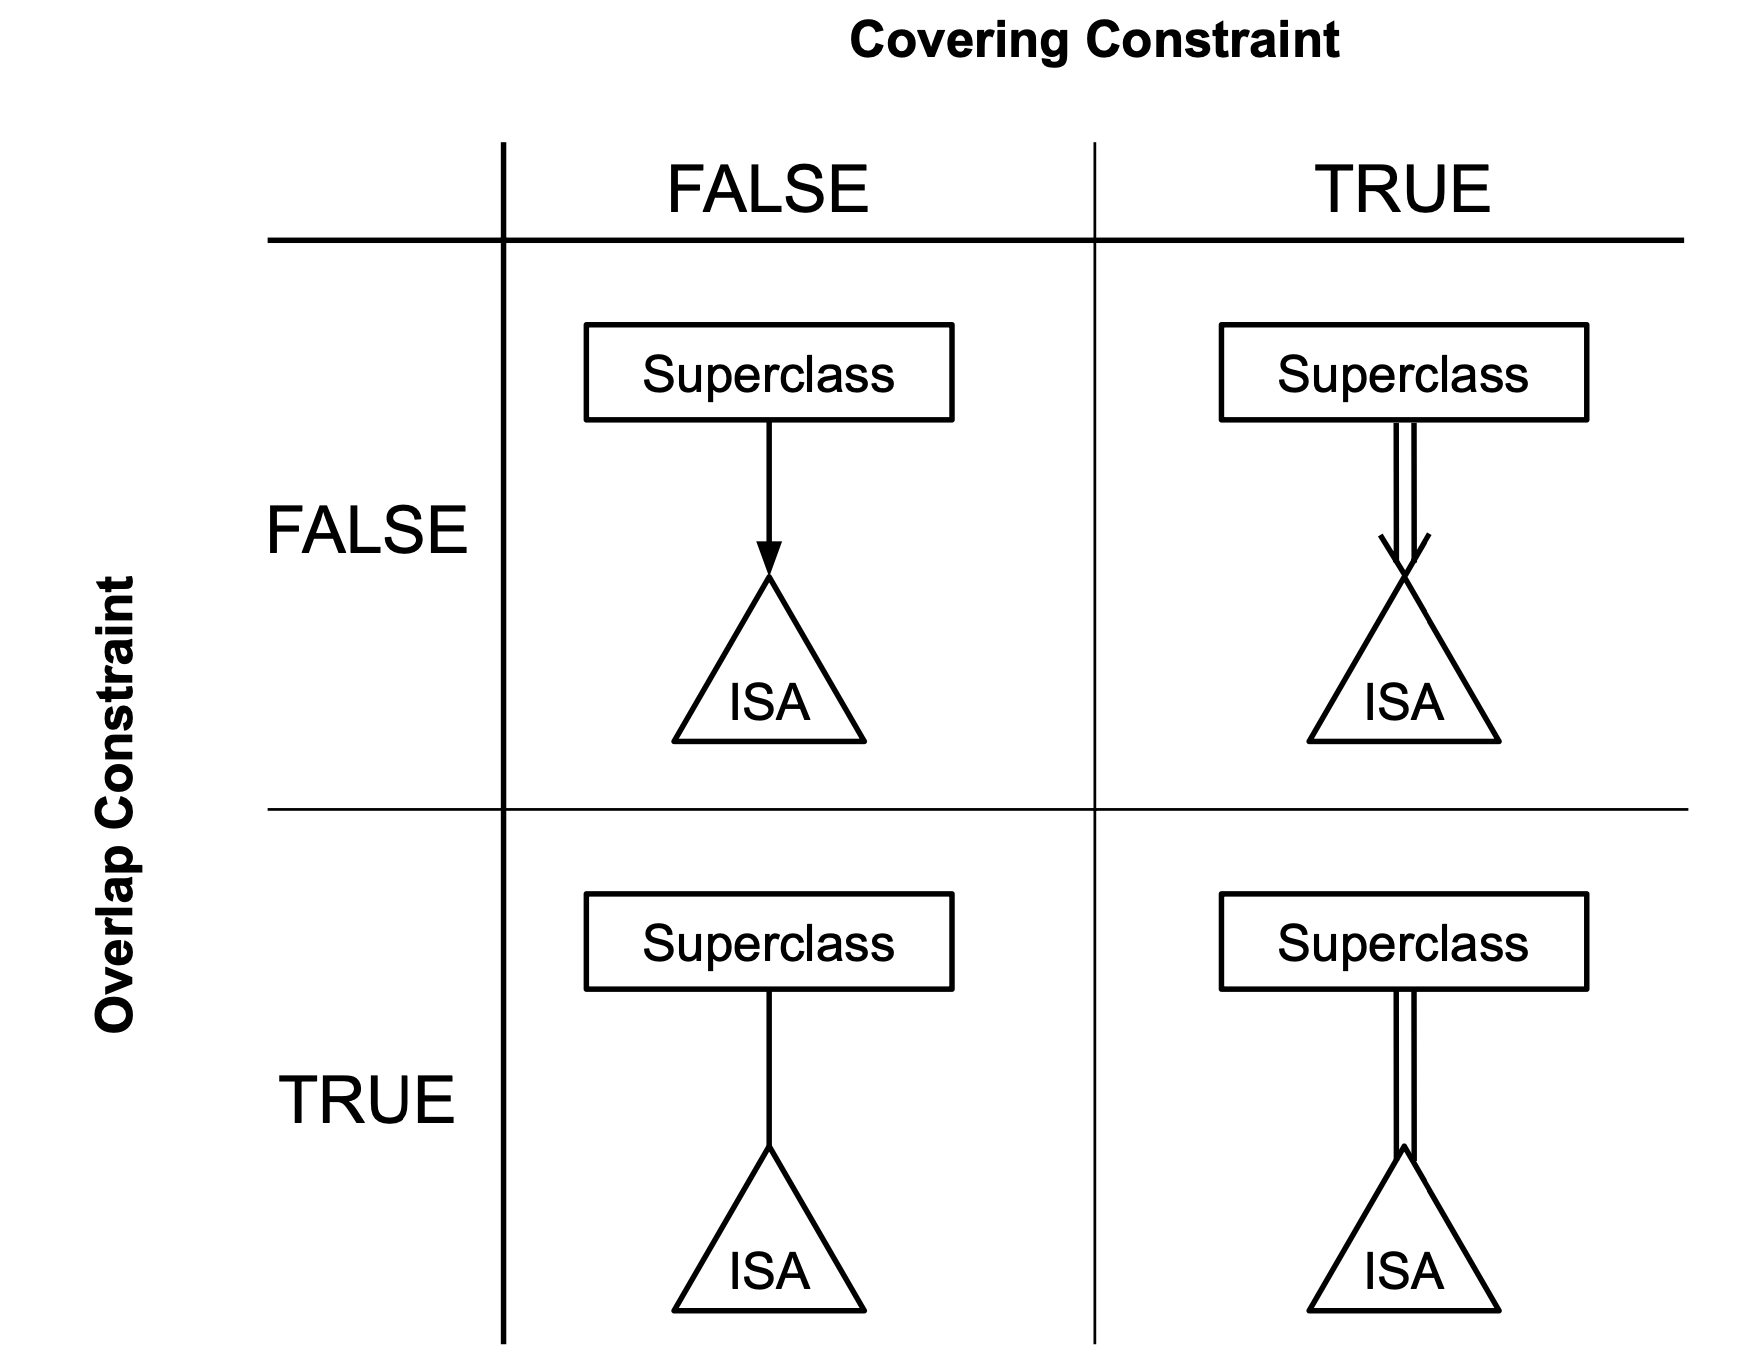
\includegraphics[width=\columnwidth]{L4/is-a-constraints}
    \end{minipage}
  \subsection*{Aggregation}
    \begin{itemize}[leftmargin=*]
      \item Abstraction that treats relationships as higher-level entities
    \end{itemize}
    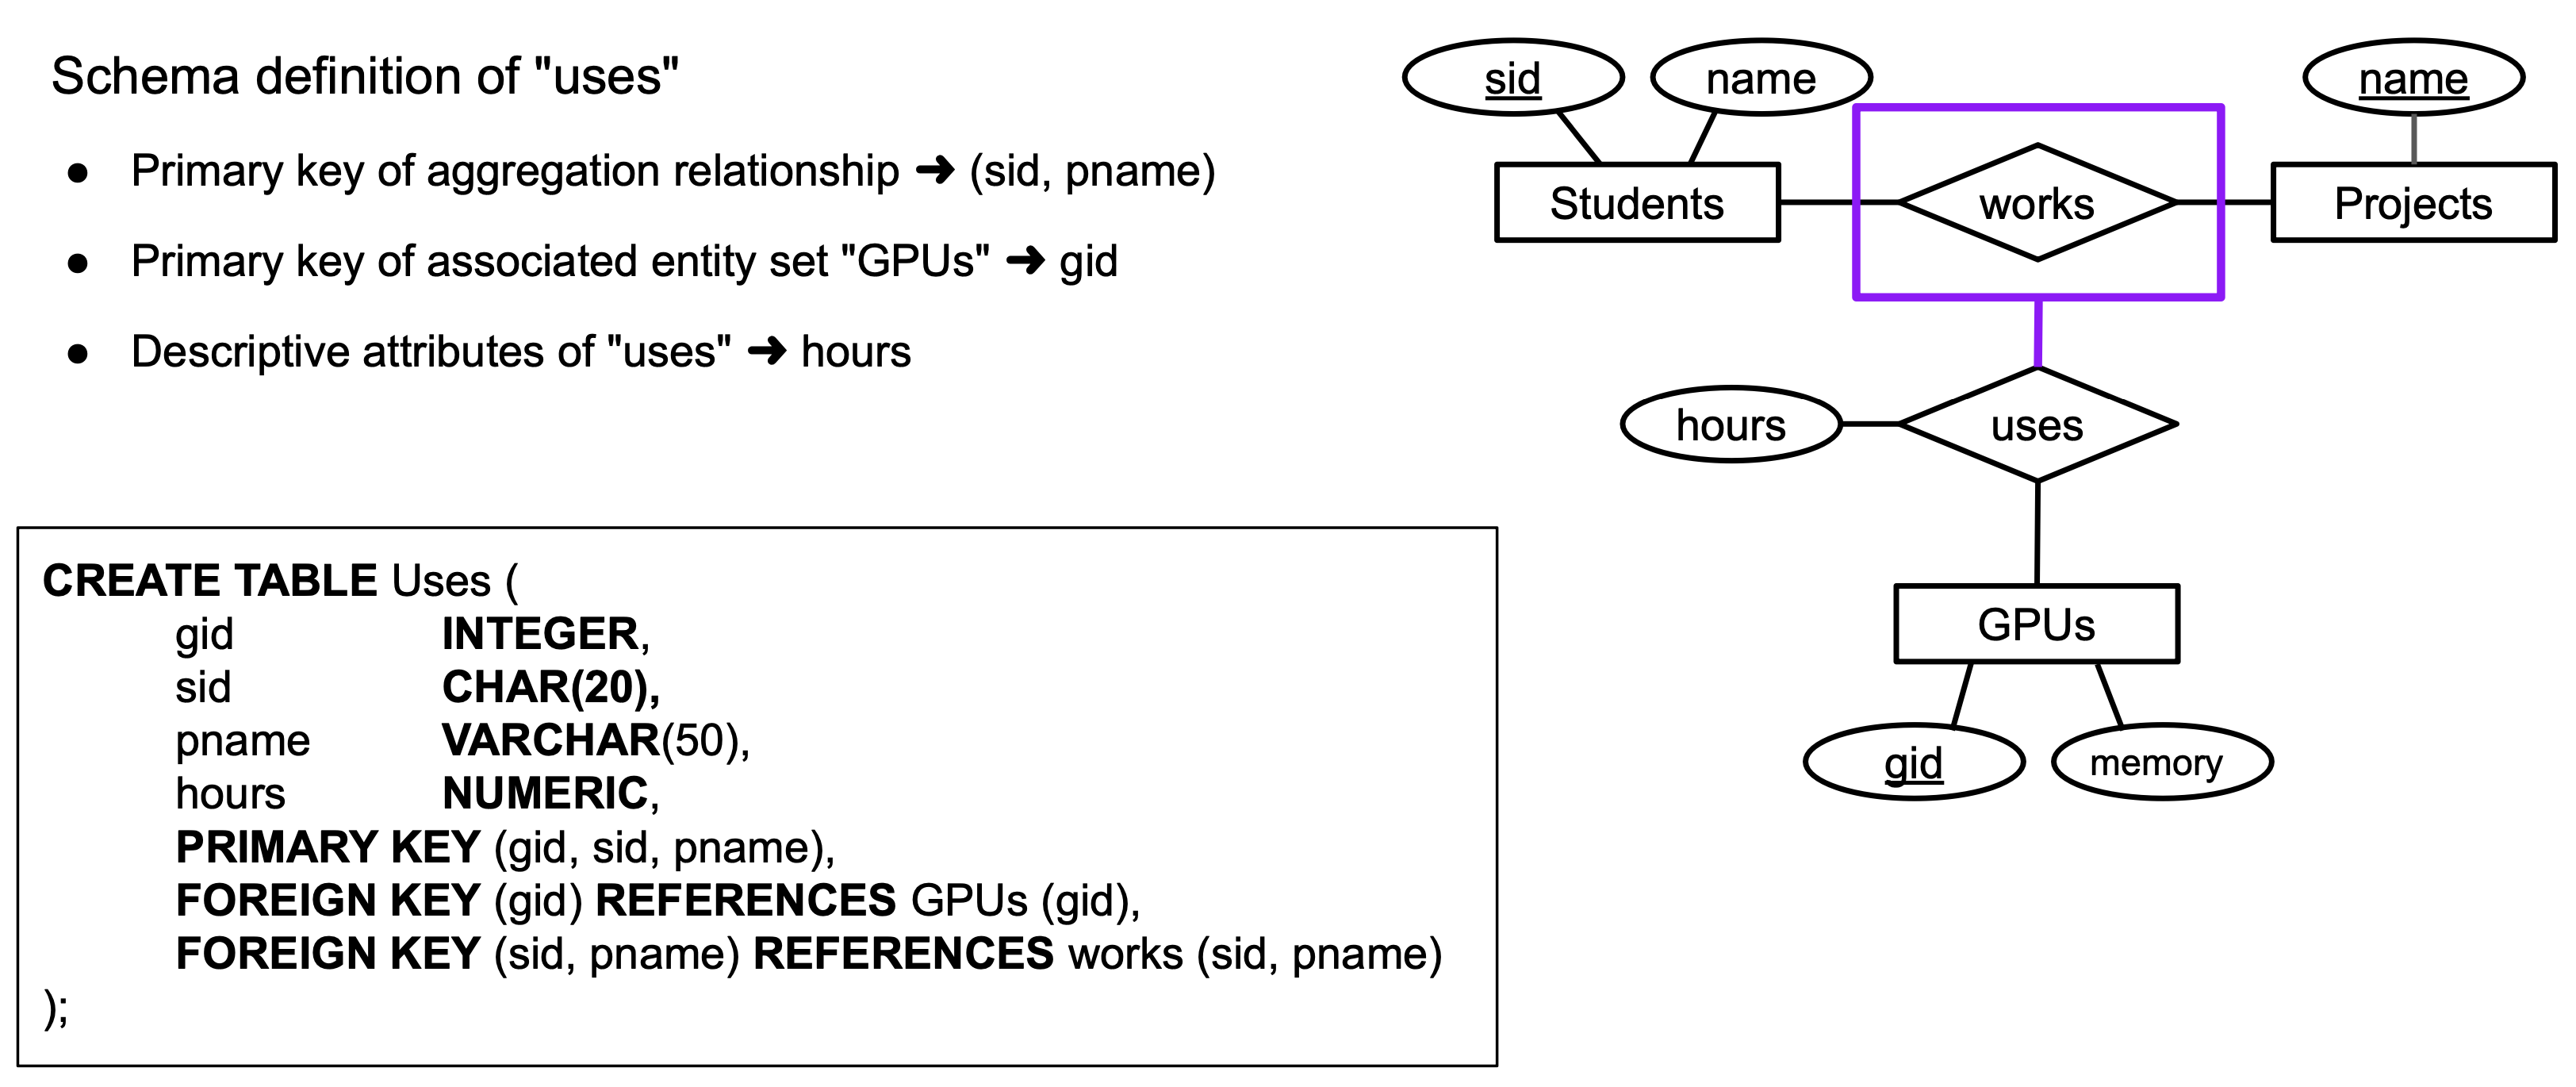
\includegraphics[width=\columnwidth]{L4/aggregation}
\section*{SQL (QUERIES)}
  \subsection*{Basic form}
    \begin{lstlisting}
SELECT DISTINCT a1, a2, ... am
FROM r1, r2, ... rm
WHERE c
    \end{lstlisting}
    corresponds to
    \[ \pi_{a_1, a_2, \cdots, a_m} (\sigma_c(r_1 \times r_2 \times \cdots \times r_n)) \]
  \subsection*{SELECT}
    \begin{itemize}[leftmargin=*]
      \item Wildcard `*' to include all attributes
      \item \ic{expr BETWEEN <lower> AND <upper>} for basic value range conditions
    \end{itemize}
    \begin{lstlisting}
SELECT * FROM countries
WHERE (continent = `Asia' OR continent = `Europe')
AND (population BETWEEN 5000000 AND 6000000)
    \end{lstlisting}
    \begin{itemize}[leftmargin=*]
      \item $\vert\vert$ for string concatenation
    \end{itemize}
    \begin{lstlisting}
-- AS is optional
SELECT name, `S$ ' || ROUND((gdp/population)*1.38)
AS gdp_per_capita FROM countries;
    \end{lstlisting}
    \begin{itemize}[leftmargin=*]
      \item \ic{SELECT DISTINCT} to eliminate duplicates
      \item Two tuples $(n_1, c_1)$ and $(n_2, c_2)$ are distinct if \\
        \ic{(n1 IS DISTINCT FROM n2) or (c1 IS DISTINCT FROM c2)} \\
        evaluates to true
    \end{itemize}
  \subsection*{WHERE}
    \begin{itemize}[leftmargin=*]
      \item Returns rows that evaluate to true
      \item Does not return rows that evaluate to unknown/null!
      \item Use \ic{IS (NOT)} \ic{NULL} for comparison with null
      \item \ic{IS (NOT)} \ic{LIKE}
        \begin{itemize}[leftmargin=*]
          \item \ic{`_'} matches single char
          \item \ic{`\%'} matches any sequence of zero or more chars
        \end{itemize}
    \end{itemize}
  \subsection*{Set operations}
    \begin{itemize}[leftmargin=*]
      \item Eliminate duplicates: \ic{UNION, INTERSECT, EXCEPT}
      \item Keep duplicates: \ic{UNION ALL, INTERSECT ALL, EXCEPT ALL}
    \end{itemize}
  \subsection*{Join operations}
    \begin{itemize}[leftmargin=*]
      \item \ic{JOIN} is interpreted as \ic{INNER JOIN}
      \item \ic{NATURAL JOIN}
      \item \ic{LEFT OUTER JOIN} interpreted as \ic{LEFT JOIN}
        \begin{itemize}[leftmargin=*]
          \item Use \ic{WHERE ... IS NULL} to get only dangling tuples
        \end{itemize}
    \end{itemize}
  \subsection*{Subqueries}
    \subsubsection*{In FROM clause}
      \begin{itemize}[leftmargin=*]
        \item Must be enclosed in parenthesis
        \item Table alias mandatory
        \item Column aliases optional
      \end{itemize}
      \begin{lstlisting}
SELECT * FROM (
  SELECT n.iso2, n.name
  FROM countries n, borders b
  WHERE n.iso2 = b.country1_iso2
  AND country2_iso2 IS NULL
) AS LandborderfreeCountries;
-- column aliases optional
-- ) AS LandborderfreeCountries(code, name);
      \end{lstlisting}
    \subsubsection*{IN subquery}
      \begin{itemize}[leftmargin=*]
        \item \ic{expr IN (subquery)}
        \item Subquery must return exactly one column
        \item Returns true if expr matches with any subquery row
        \item \ic{IN} can typically be replaced with inner joins
        \item \ic{NOT IN} can typically be replaced with outer joins
      \end{itemize}
      \begin{lstlisting}
-- subquery is a SELECT
SELECT * FROM countries WHERE name IN (SELECT name FROM cities);
-- subquery is a manually specified result of a subquery
SELECT * FROM countries WHERE continent IN (`Asia', `Europe');
      \end{lstlisting}
    \subsubsection*{ANY/SOME subquery}
      \begin{itemize}[leftmargin=*]
        \item \ic{expr op ANY (subquery)}
        \item Subquery must return exactly one column
        \item Expression is compared to each subquery row using operator \ic{op}
        \item Returns true if comparison evaluates to TRUE for at least one subquery row
        \item \ic{.. < ANY(..)} $\Rightarrow$ Not maximum
        \item \ic{.. > ANY(..)} $\Rightarrow$ Not minimum
      \end{itemize}
    \subsubsection*{ALL subquery}
      \begin{itemize}[leftmargin=*]
        \item \ic{expr op ANY (subquery)}
        \item Subquery must return exactly one column
        \item Expression is compared to each subquery row using operator \ic{op}
        \item Returns true if comparison evaluates to TRUE for all subquery rows
        \item \ic{.. <= ALL(..)} $\Rightarrow$ Minimum
        \item \ic{.. >= ALL(..)} $\Rightarrow$ Maximum
      \end{itemize}
    \subsubsection*{EXISTS subqueries}
      \begin{itemize}[leftmargin=*]
        \item \ic{EXISTS (subquery)}
        \item Returns TRUE if subquery returns at least one tuple
        \item Generally correlated. If uncorrelated, then likely either wrong or unnecessary
      \end{itemize}
    \subsubsection*{Correlated subqueries}
      \begin{itemize}[leftmargin=*]
        \item Uses value from outer query
        \item Result of subquery depends on value of outer query
          \begin{itemize}[leftmargin=*]
            \item Potentially slow performance
            \item For \ic{ALL} condition, problematic if subquery contains NULL value, since condition never evaluates to TRUE
            \item Potential naming ambiguities - use table aliases
          \end{itemize}
      \end{itemize}
      \paragraph{Scoping rules}
        \begin{itemize}[leftmargin=*]
          \item (Scope applies inwards) Table alias decalred in subquery Q can only be used in Q, or subqueries nested within Q
          \item If same table alias is declared in subquery Q and in an outer query, then use the declaration in Q
        \end{itemize}
    \subsubsection*{Scalar subqueries}
      \begin{itemize}[leftmargin=*]
        \item Occurs when subquery returns a single value (1 row, 1 column)
        \item Can be used as expression in queries
      \end{itemize}
    \subsubsection*{Row constructors}
      \begin{itemize}[leftmargin=*]
        \item Allow subqueries to return more than one attribute
        \item Number of attributes in row constructor must match the one of the subquery
      \end{itemize}
      \begin{lstlisting}
SELECT name, population, gdp FROM countries
WHERE ROW(population, gdp) > ANY (SELECT population, gdp
                                  FROM countries
                                  WHERE name in (`Germany', `France'));
      \end{lstlisting}
      \begin{itemize}[leftmargin=*]
        \item If comparison op is \ic{=} or \ic{<>}, then tuple comparison works as expected
        \item However, for \ic{<, <=, >, >=}, the row elements are compared left-to-right, stopping as soon as an unequal or null pair of elements is found
          \begin{itemize}[leftmargin=*]
            \item If either of this pair of elements is null, the result of the row comparison is unknown (null)
            \item Otherwise comparison of this pair of elements determines the result
          \end{itemize}
        \item Can use \ic{SELECT ROW(...) op ROW(...) as res} to test the functionality
      \end{itemize}
    \subsubsection*{Equivalent subqueries}
      \begin{itemize}[leftmargin=*]
        \item \ic{expr IN (subquery)} $\equiv$ \ic{expr = ANY (subquery)}
        \item \ic{expr1 op ANY(SELECT expr2 FROM ... WHERE ...)} $\equiv$ \\
          \ic{EXISTS(SELECT * FROM ... WHERE ... AND expr1 op expr2)}
      \end{itemize}
  \subsection*{Sorting}
    \begin{itemize}[leftmargin=*]
      \item \ic{ORDER BY attribute ASC (DESC)}
      \item \ic{ORDER BY attr1 ASC, attr2 DESC} - 2nd sorting criteria only affects result if 1st sorting criteria has ambiguity
    \end{itemize}
  \subsection*{Ranking}
    \begin{itemize}[leftmargin=*]
      \item \ic{LIMIT k}: return first $k$ tuples of the result table
      \item \ic{OFFSET k}: specify the position of the first tuple to be considered
      \item Used with \ic{ORDER BY}
      \item \ic{ORDER BY ... OFFSET 5 LIMIT 5} - get 6th to 10th tuples in sorting criteria
    \end{itemize}
\section*{SQL (Aggregation)}
  \begin{itemize}[leftmargin=*]
    \item Computes a single value, given a set of tuples
    \item e.g. \ic{MIN(), MAX(), AVG(), COUNT(), SUM()}
    \item \ic{MIN(A)} does not consider null values for attribute $A$
  \end{itemize}
  \subsection*{Signatures}
    \begin{itemize}[leftmargin=*]
      \item \ic{MIN, MAX} defined for all data types, returns same type as input
      \item \ic{SUM} defined for all numeric data types
        \begin{itemize}[leftmargin=*]
          \item 
            \begin{hlist}
              \item \ic{SUM(INTEGER) -> BIGINT}
              \item \ic{SUM(REAL) -> REAL}
            \end{hlist}
        \end{itemize}
      \item \ic{COUNT} defined for all data types; returns \ic{BIGINT}
    \end{itemize}
  \subsection*{Handling NULL} \noindent
    Let $R$ be a non-empty relation with attribute $A$.
    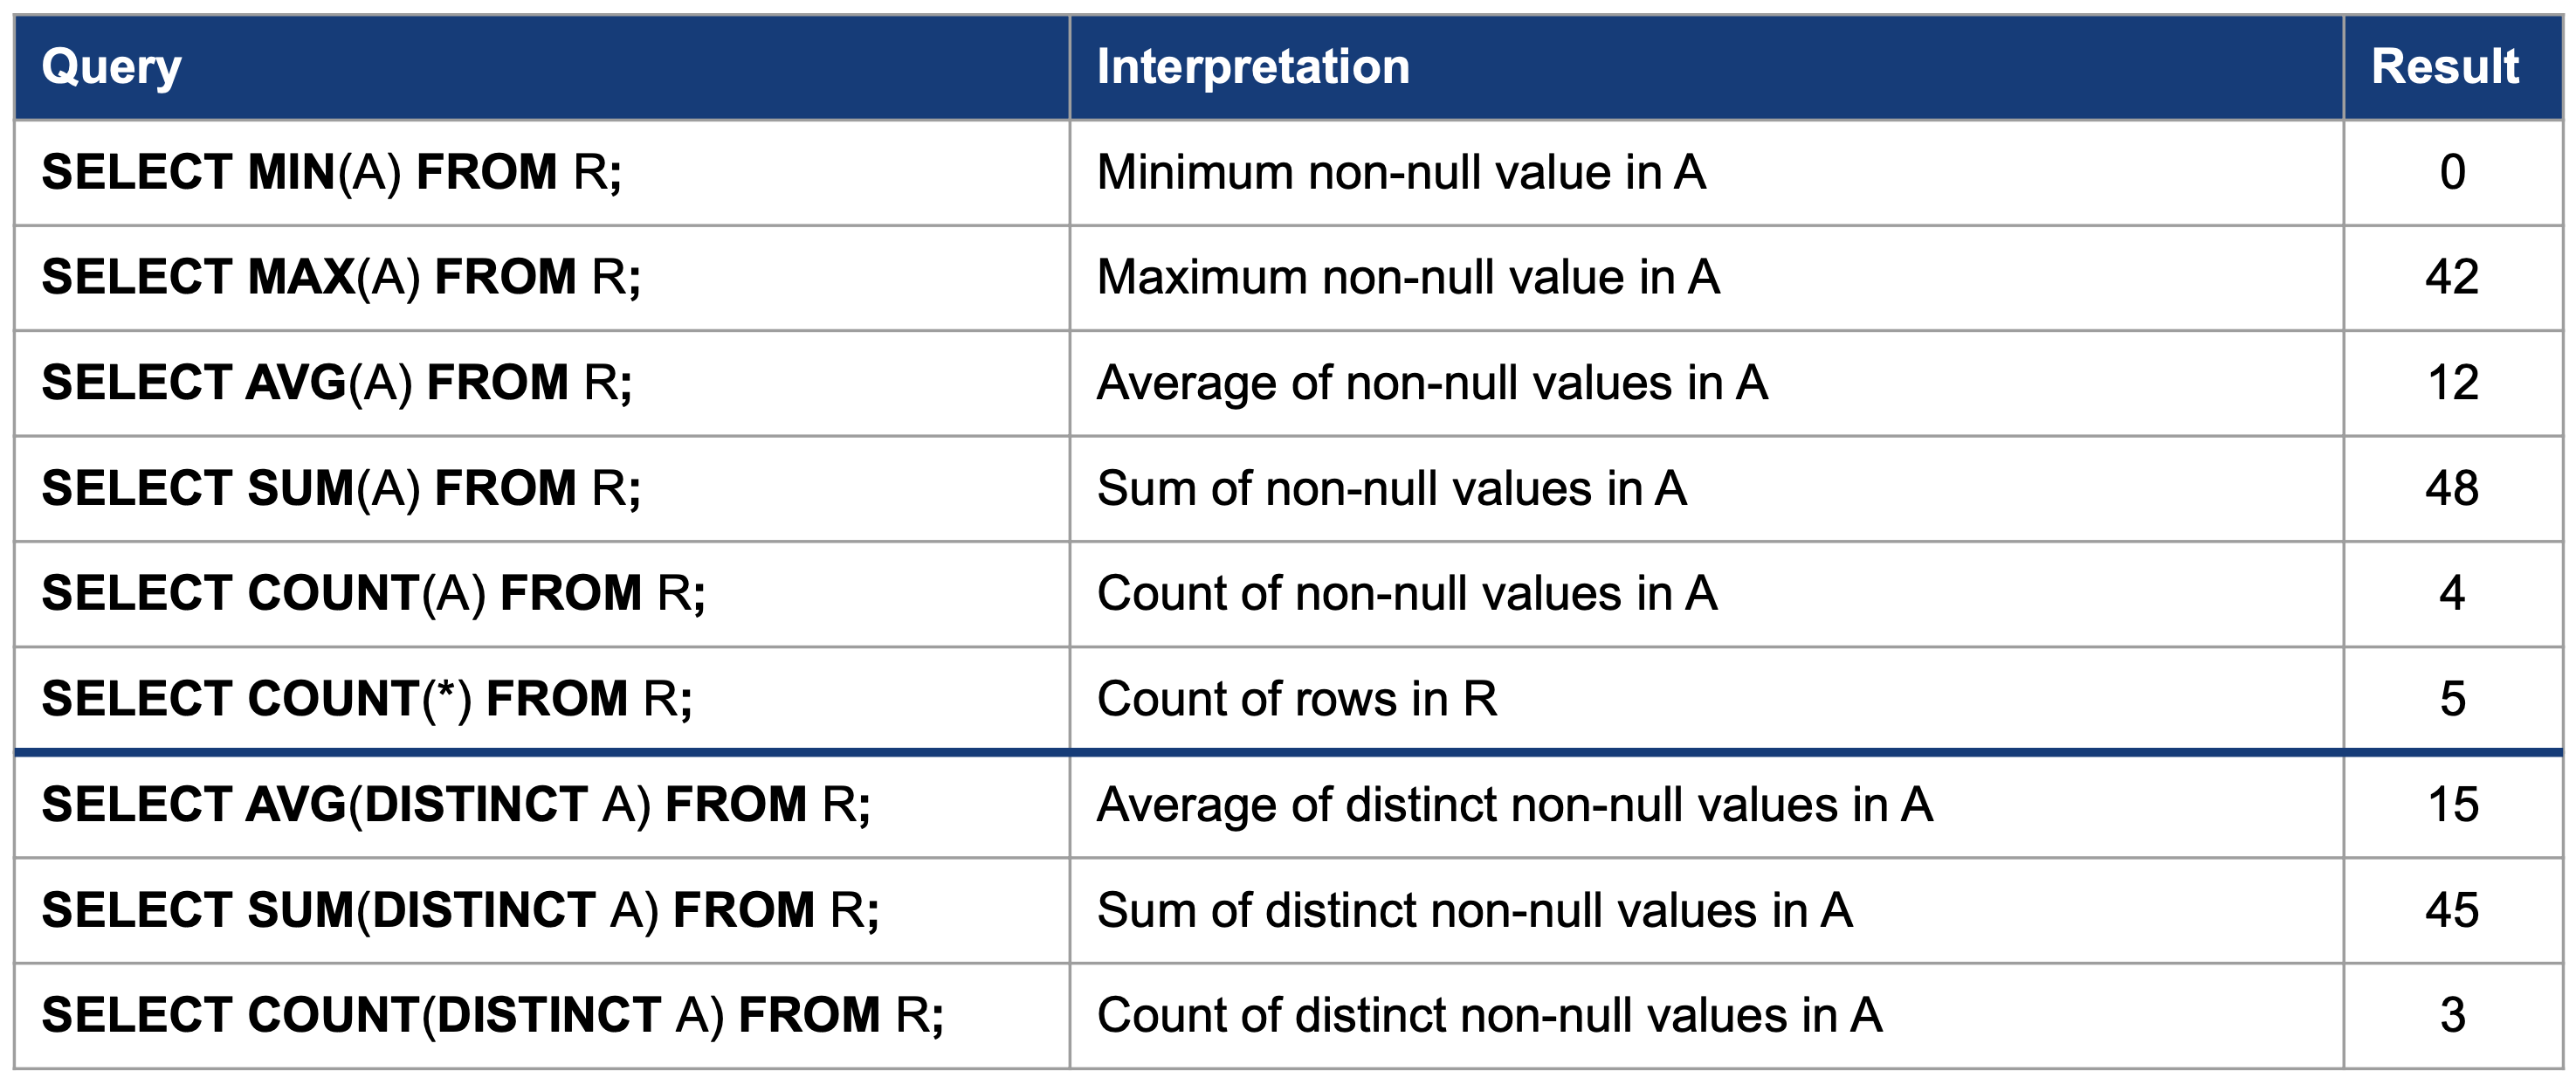
\includegraphics[width=\columnwidth]{L6/aggregate-null}
    Let $R, S$ be two relations with an attribute $A$,
    \begin{itemize}[leftmargin=*]
      \item where $R$ is an empty relation, and
      \item $S$ is a non-empty relation with $n$ tuples, only null values for $A$
    \end{itemize}
    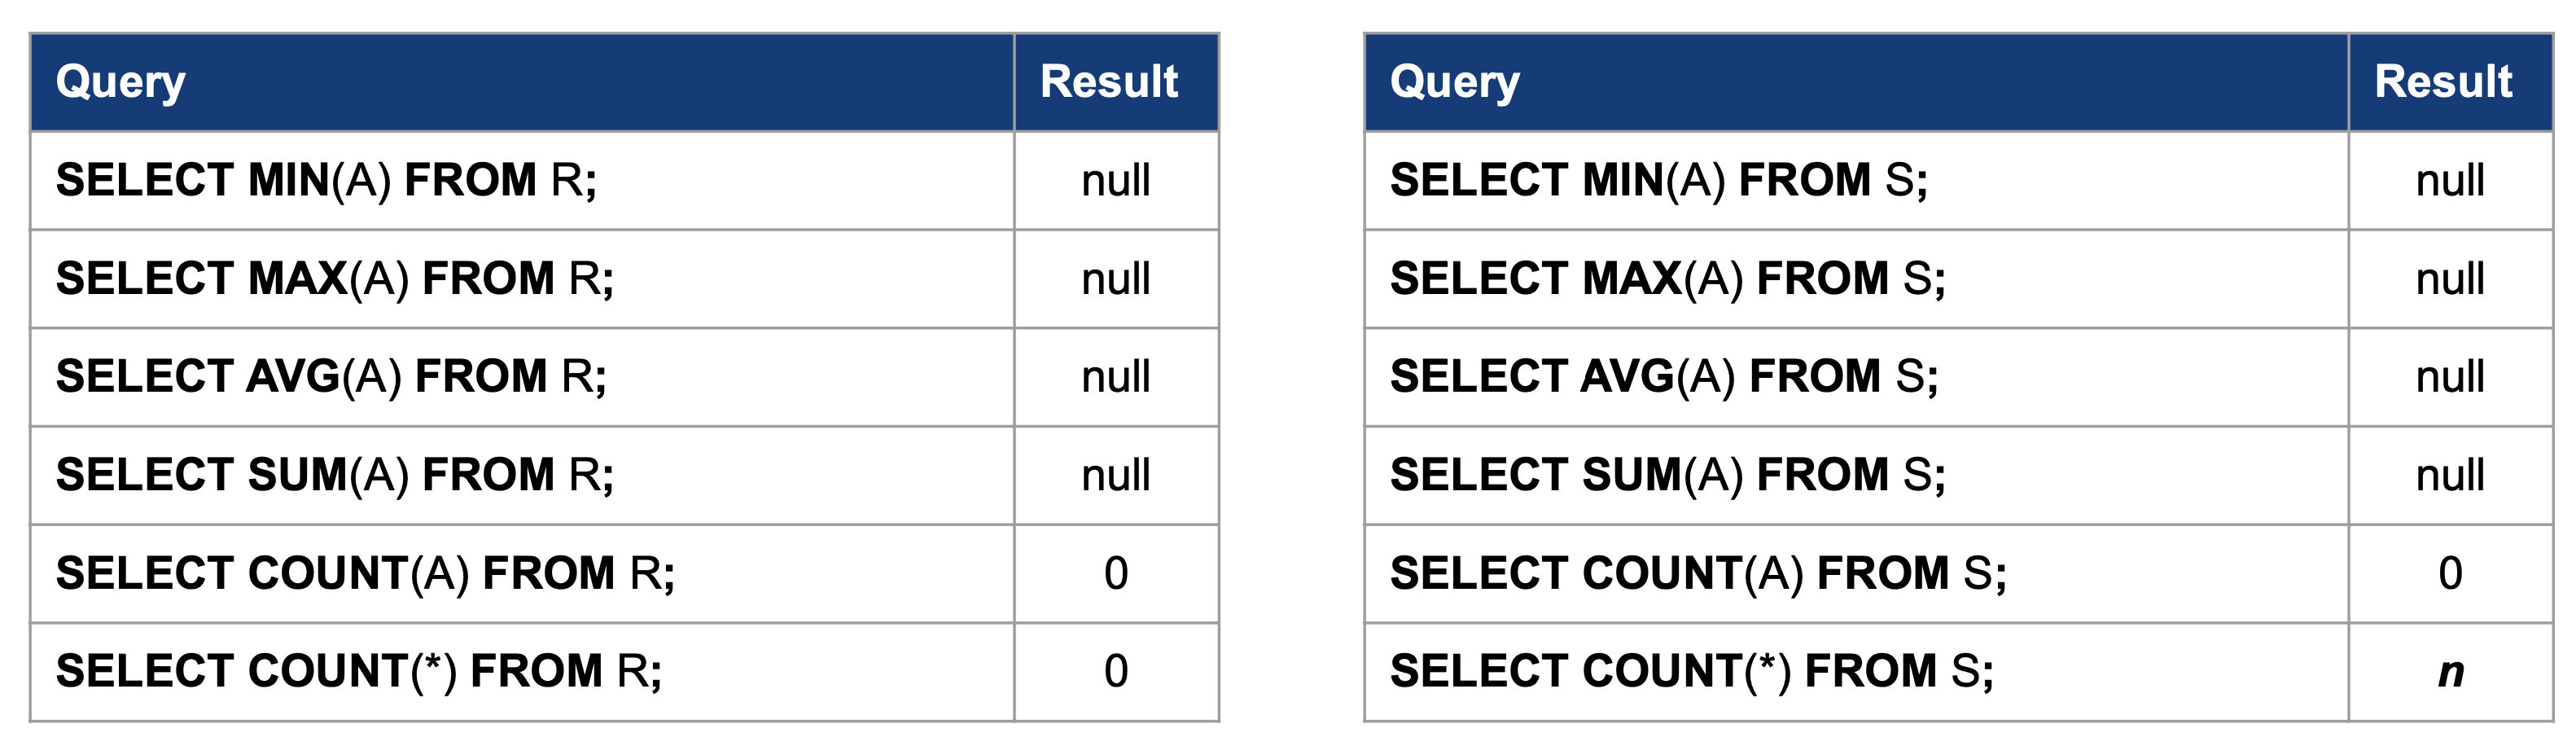
\includegraphics[width=\columnwidth]{L6/aggregate-null-2}
  \subsection*{Grouping}
    \begin{itemize}[leftmargin=*]
      \item Logical partition of relation into groups, based on values for specified attributes
      \item Aggregate function applied over group, so 1 result tuple for each group
      \item Given \ic{GROUP BY a1, a2, .. an}, 2 tuples $x$ and $y$ belong to the same group if for all $k \in \{1 .. n\}$, \ic{x.ak IS NOT DISTINCT FROM y.ak} evaluates to TRUE
        \begin{itemize}[leftmargin=*]
          \item i.e. NULL is treated as a value
        \end{itemize}
      \item If column $A$ of table $R$ appears in \ic{SELECT} clause, one of the following conditions must hold:
        \begin{enumerate}[leftmargin=*]
          \item $A$ appears in the \ic{GROUP BY} clause
          \item $A$ appears as input of an aggregation function in the \ic{SELECT} clause
          \item Primary key of $R$ appears in the \ic{GROUP BY} clause
        \end{enumerate}
    \end{itemize}
    \begin{lstlisting}
-- find lowest, highest, overall population size for each continent
SELECT continent,
  MIN(population) AS lowest,
  MAX(population) AS highest,
  SUM(population) AS overall
FROM countries
GROUP BY continent;
    \end{lstlisting}
  \subsection*{Having}
    \begin{itemize}[leftmargin=*]
      \item Conditions check for each group defined by \ic{GROUP BY} clause
      \item Must be used with \ic{GROUP BY}
      \item If column $A$ of table $R$ appears in \ic{HAVING} clause, one of the following conditions must hold:
        \begin{enumerate}[leftmargin=*]
          \item $A$ appears in the \ic{GROUP BY} clause
          \item $A$ appears as input of an aggregation function in the \ic{HAVING} clause
          \item Primary key of $R$ appears in the \ic{GROUP BY} clause
        \end{enumerate}
    \end{itemize}
    \begin{lstlisting}
-- Find all routes served by >12 airlines
SELECT from_code, to_code, COUNT(*) AS num_airlines
FROM routes GROUP BY from_code, to_code HAVING COUNT(*) > 12;
    \end{lstlisting}
  \subsection*{Conceptual evaluation of queries} \noindent
    FROM $\rightarrow$ WHERE $\rightarrow$ GROUP BY $\rightarrow$ HAVING $\rightarrow$ SELECT $\rightarrow$ ORDER BY $\rightarrow$ LIMIT/OFFSET
\section*{SQL (Conditionals)}
  \subsection*{CASE expression}
    \begin{itemize}[leftmargin=*]
      \item Generic conditional, like if/else statements
      \item Used in SELECT, ORDER BY, etc
    \end{itemize}
    \begin{minipage}{0.475 \columnwidth}
      \begin{center}
        Regular if-else
        \begin{lstlisting}
CASE
  WHEN cond1 then res1
  WHEN cond2 then res2
  ...
  WHEN condN then resN
  ELSE res0
END
        \end{lstlisting}
      \end{center}
    \end{minipage}
    \begin{minipage}{0.475 \columnwidth}
      \begin{center}
        Switch-like statement
        \begin{lstlisting}
CASE expression
  WHEN val1 then res1
  WHEN val2 then res2
  ...
  WHEN valN then resN
  ELSE res0
END
        \end{lstlisting}
      \end{center}
    \end{minipage}
  \subsection*{COALESCE}
    \begin{itemize}[leftmargin=*]
      \item Returns first non-NULL value in list of input args
      \item Returns NULL if lit of input args are NULL
    \end{itemize}
    \begin{lstlisting}
-- if NULL, then set type to other
SELECT type, COUNT(*) AS city_ount
FROM
  (SELECT COALESCE(type, `other') AS type
   FROM cities) t
GROUP BY type;
    \end{lstlisting}
  \subsection*{NULLIF}
    \begin{itemize}[leftmargin=*]
      \item \ic{NULLIF(v1, v2)} returns NULL if $v_1 = v_2$, otherwise returns $v_1$
      \item Common use case: convert special values (zero, empty string) to NULL values
    \end{itemize}
    \begin{lstlisting}
-- Unknown values are represented as 0
-- so set them to NULL for aggregation to ignore
SELECT MIN(NULLIF(gini, 0)) AS min_gini,
       AVG(NULLIF(gini, 0)) AS avg_gini,
FROM countries;
    \end{lstlisting}
\section*{SQL (Structuring Queries)}
  \subsection*{Common Table Expressions (CTEs)}
    \begin{itemize}[leftmargin=*]
      \item Temporarily named query
      \item Multiple CTEs can be used within an SQL statement
      \item CTEs can refer previous CTEs, or can be not referred at all
      \item Improves readabiliity, debugging, maintenance
    \end{itemize}
    \begin{minipage}{0.3 \columnwidth}
      \begin{center}
        General syntax
        \begin{lstlisting}
WITH
  C1 AS (Q1),
  C2 AS (Q2),
  ...
  CN as (QN),
SQL statement S;
        \end{lstlisting}
      \end{center}
    \end{minipage}
    \begin{minipage}{0.675 \columnwidth}
      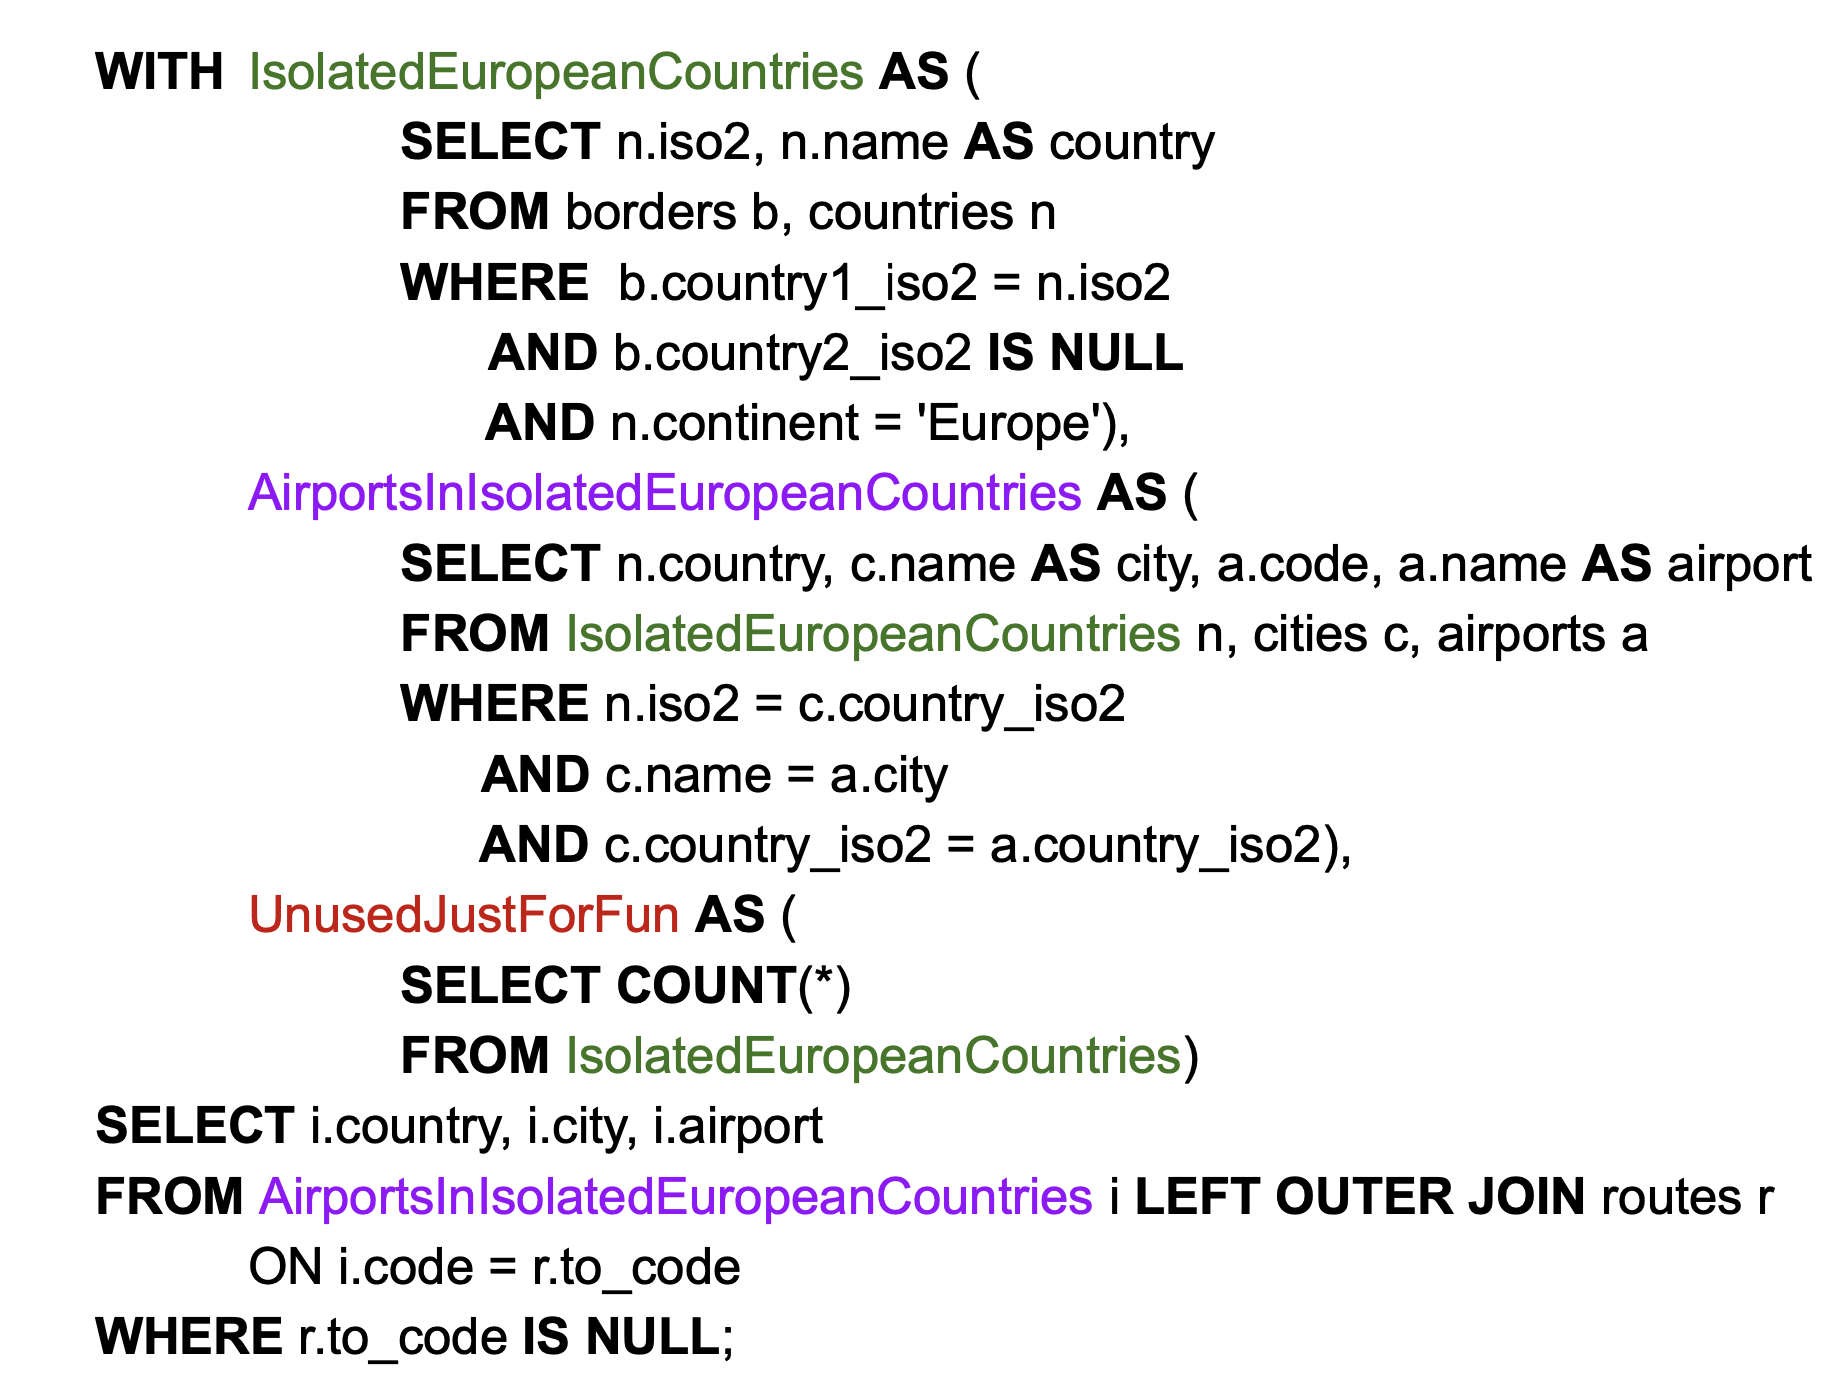
\includegraphics[width=\columnwidth]{L6/cte}
    \end{minipage}
    \begin{itemize}[leftmargin=*]
      \item Each $C_i$ is the name of a temporary table defined by $Q_i$
      \item Each $C_i$ can reference any other $C_j$ that has been declared before $C_i$
      \item SQL statement $S$ can reference any possible subset of all $C_i$
    \end{itemize}
  \subsection*{Views}
    \begin{itemize}[leftmargin=*]
      \item Permanently named query (virtual table)
        \begin{itemize}[leftmargin=*]
          \item Query is stored (not result), and re-executed each time view is used
        \end{itemize}
      \item Can be used like normal tables
        \begin{itemize}[leftmargin=*]
          \item No restriction when used in \ic{SELECT} statements
          \item Restrictions for \ic{INSERT, UPDATE, DELETE} (updatable view)
        \end{itemize}
    \end{itemize}
    \subsubsection*{Updatable view requirements} \noindent
      Satisfy all of
      \begin{enumerate}[leftmargin=*]
        \item Must have exactly 1 entry in its \ic{FROM} list, which must be a table, or another updatable view
        \item Can only update one attribute of a particular row at a time
        \item No \ic{WITH, DISTINCT, GROUP BY, HAVING, LIMIT, OFFSET}
        \item No set operations \ic{UNION, INTERSECT, EXCEPT}
        \item No aggregate functions
        \item No constraint violations
      \end{enumerate}
    \begin{lstlisting}
CREATE VIEW view_name AS
SELECT .. FROM .. WHERE .. GROUP BY ..;
    \end{lstlisting}
  \subsection*{Universal quantification}
    \begin{itemize}[leftmargin=*]
      \item No support for universal quantification (e.g. find names of all users that have visited all countries)
      \item Transform query using logical equivalences
        \begin{itemize}[leftmargin=*]
          \item There does not exist a country that the user has not visited
        \end{itemize}
      \item Alternative interpretation
        \begin{itemize}[leftmargin=*]
          \item Number of tuples in Visited for that user must match total number of countries
        \end{itemize}
    \end{itemize}
    \subsubsection*{Logical equivalences} \noindent
      \begin{itemize}[leftmargin=*]
        \item Can be used for other types of queries
        \item e.g. $p \implies q \equiv {}^\sim p \lor q$
      \end{itemize}
  \subsection*{Recursive queries}
    \begin{itemize}[leftmargin=*]
      \item Using CTEs
    \end{itemize}
    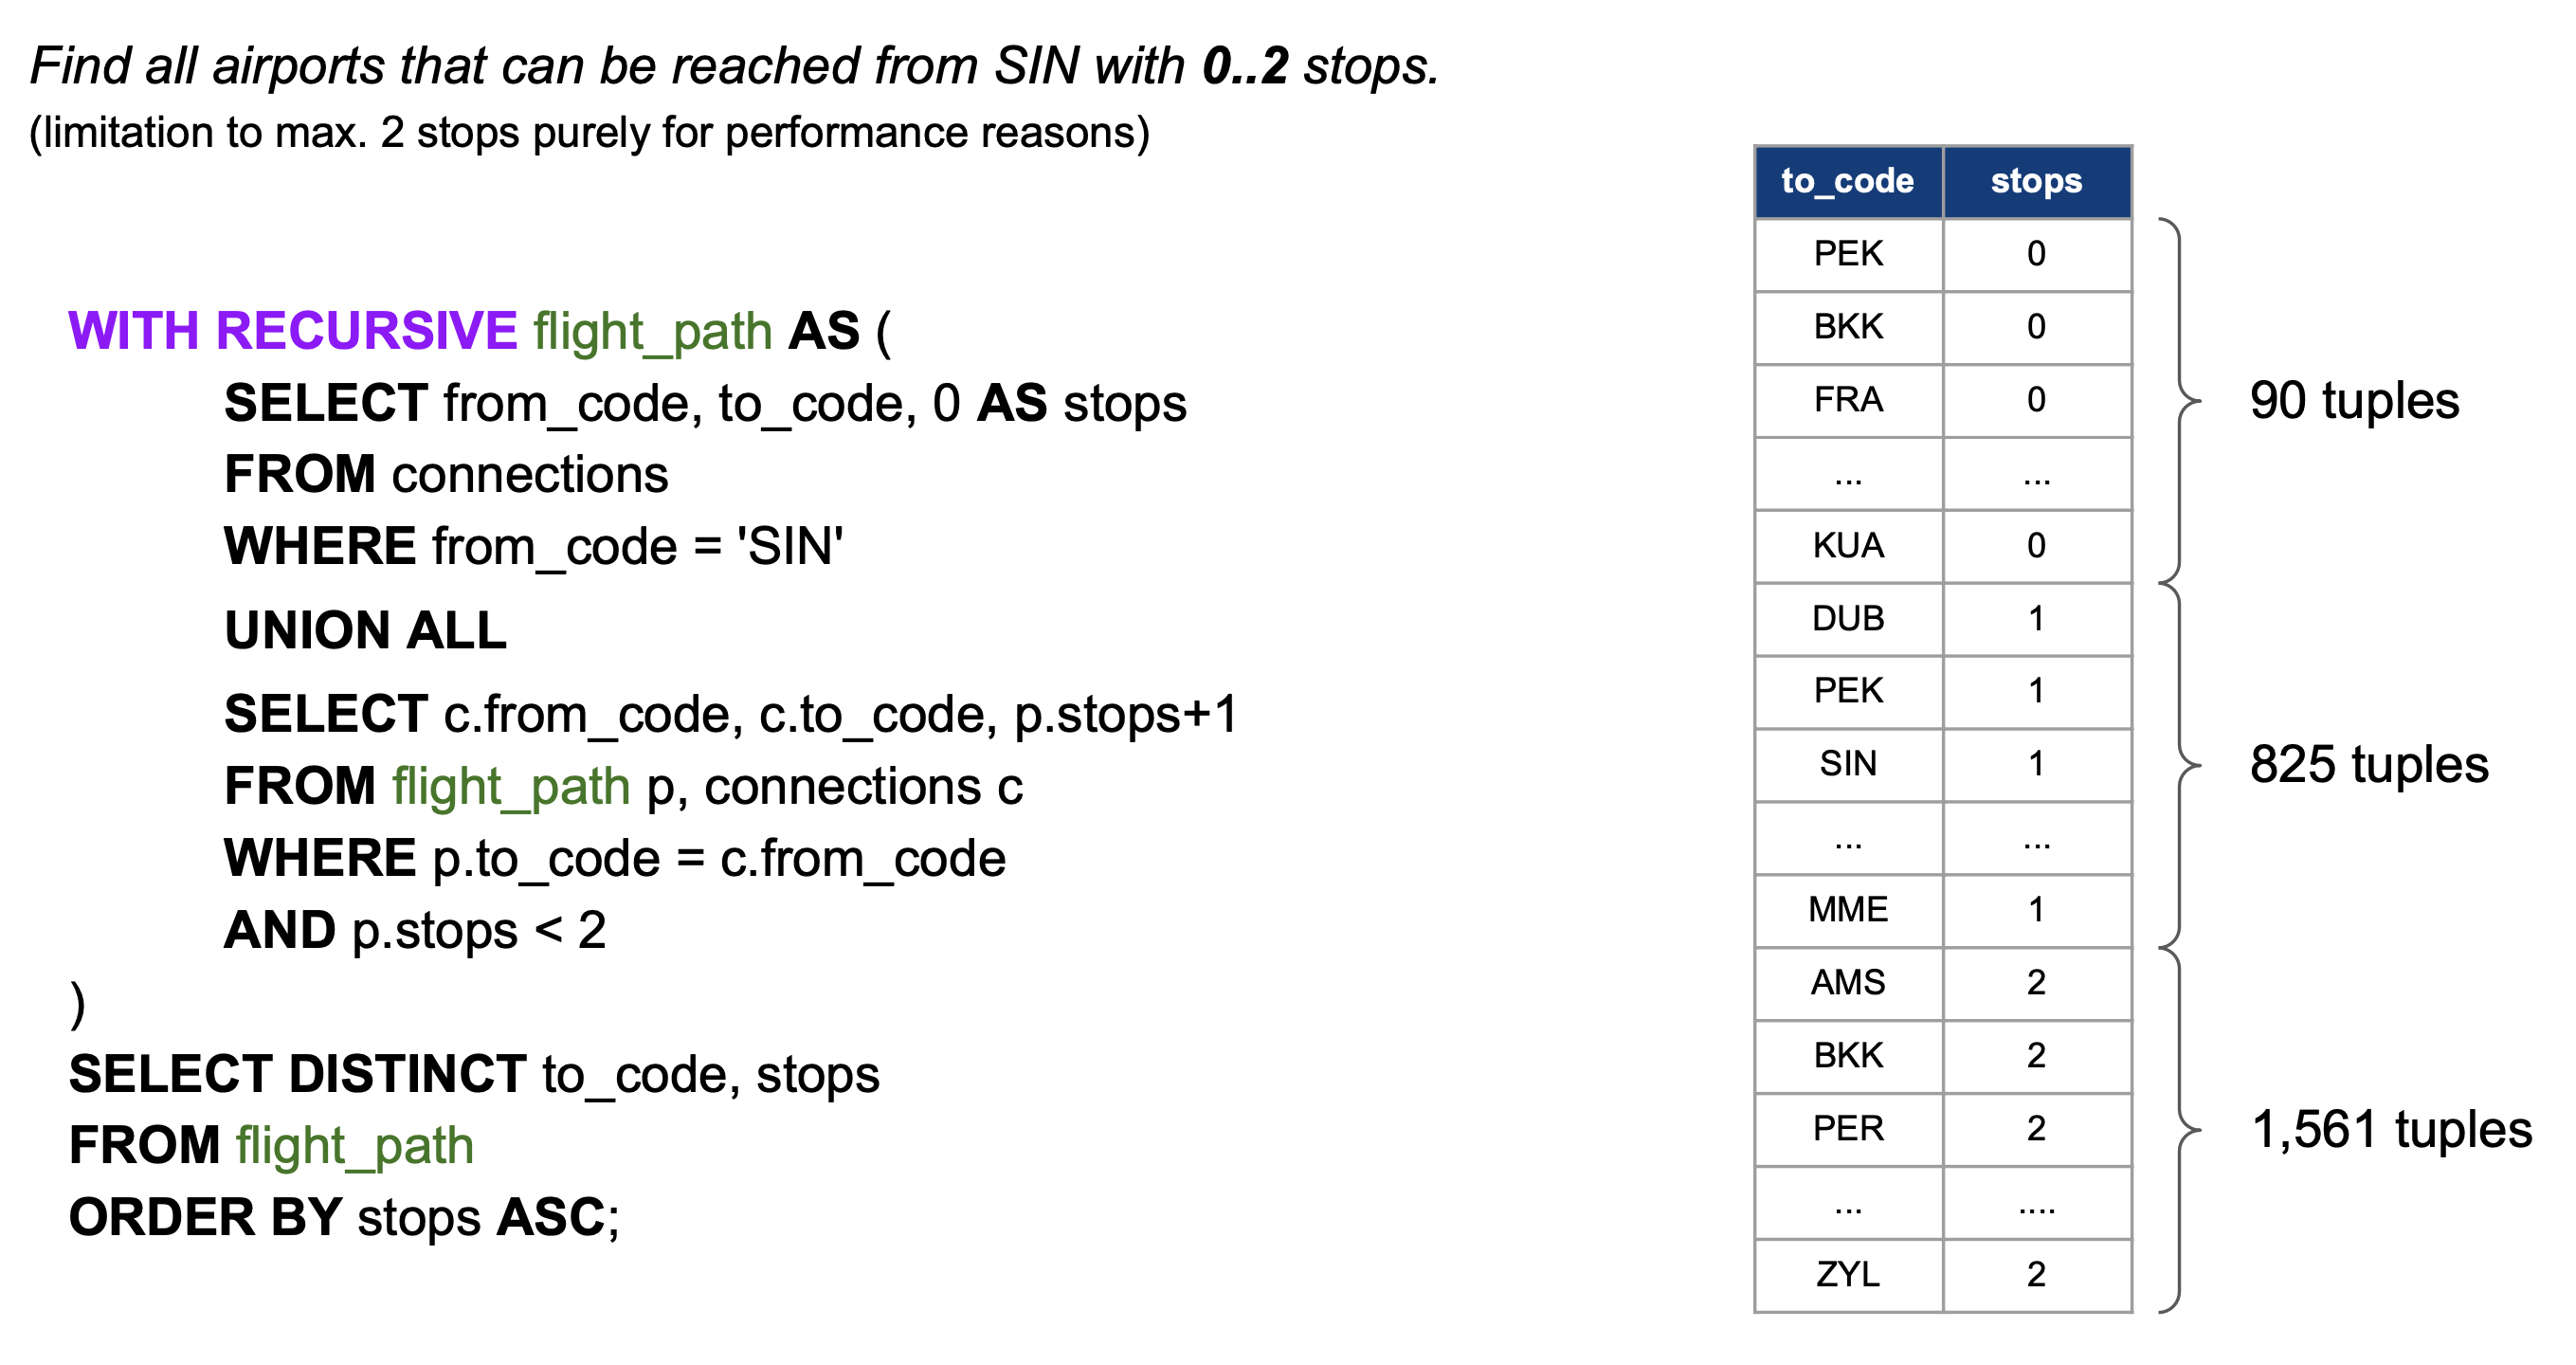
\includegraphics[width=\columnwidth]{L6/recursive}
\end{multicols*}
\end{document}
